\documentclass[pdflatex,11pt]{aghdpl}
% \documentclass{aghdpl}               % przy kompilacji programem latex
% \documentclass[pdflatex,en]{aghdpl}  % praca w języku angielskim
\usepackage[polish]{babel}
\usepackage[utf8]{inputenc}

% dodatkowe pakiety
\usepackage{enumerate}
\usepackage{listings}
\usepackage{color}
\lstloadlanguages{TeX}

\lstset{
  literate={ą}{{\k{a}}}1
           {ć}{{\'c}}1
           {ę}{{\k{e}}}1
           {ó}{{\'o}}1
           {ń}{{\'n}}1
           {ł}{{\l{}}}1
           {ś}{{\'s}}1
           {ź}{{\'z}}1
           {ż}{{\.z}}1
           {Ą}{{\k{A}}}1
           {Ć}{{\'C}}1
           {Ę}{{\k{E}}}1
           {Ó}{{\'O}}1
           {Ń}{{\'N}}1
           {Ł}{{\L{}}}1
           {Ś}{{\'S}}1
           {Ź}{{\'Z}}1
           {Ż}{{\.Z}}1
}

%---------------------------------------------------------------------------

\author{Mateusz Urbanik}
\shortauthor{M. Urbanik}

\titlePL{Opracowanie metod optymalizacji kosztów leczenia pacjenta przy użyciu technologii informatycznych}
\titleEN{Developing methods to optimize patient treatment costs, using information technology}

\shorttitlePL{Optymalizacja kosztów leczenia pacjenta} % skrócona wersja tytułu jeśli jest bardzo długi
\shorttitleEN{Optimization of patient treatment costs}

\thesistypePL{Praca magisterska}
\thesistypeEN{Master of Science Thesis}

\supervisorPL{dr inż. Rafał Mrówka}
\supervisorEN{Rafał Mrówka D.}

\date{2012}

\departmentPL{Katedra Automatyki}
\departmentEN{Department of Automatics}

\facultyPL{Wydział Elektrotechniki, Automatyki, Informatyki i Elektroniki}
\facultyEN{Faculty of Electrical Engineering, Automatics, Computer Science and Electronics}

\acknowledgements{Serdecznie dziękuję \dots tu ciąg dalszych podziękowań np. dla promotora, żony, sąsiada itp.}



\setlength{\cftsecnumwidth}{10mm}

%---------------------------------------------------------------------------

\begin{document}

\titlepages

\tableofcontents
\clearpage

% \include{rozdzial1}
% \include{rozdzial2}
\chapter{Wstęp}
\label{cha:wstep}

Rozliczanie kosztów leczenia pacjenta jest problemem skomplikowanym. Z jednej strony dążymy do rozwiązania, w~którym kluczowym czynnikiem jest zdrowie pacjenta. Aspekt medyczny brany jest pod uwagę na pierwszym miejscu. Jednak z drugiej strony równie ważnym jest aspekt finansowy. Nieprawidłowo działający system rozliczeń ma bezpośredni wpływ na aspekt medyczny, co przekłada się na niską jakość świadczonych usług\cite{kozierkiewicz_jgp}. Należy więc oczekiwać, że przyjęta przez płatnika metoda finansowania świadczeń opieki zdrowotnej powinna dążyć do zapewnienia obiektywnego pomiaru kosztów leczenia w~jednostkach szpitalnych. Jednocześnie powinna motywować świadczeniodawców do zwiększania dostępności do odpowiedniej jakości świadczeń, jak również ograniczać nieuzasadniony wzrost kosztów opieki zdrowotnej.

Dotychczasowe doświadczenia światowe wskazują, że najlepszą metodą finansowania świadczeń medycznych jest system Jednorodnych Grup Pacjentów\cite{kozierkiewicz_jgp}. Łączy on zarówno aspekt medyczny jak i finansowy. Istotnym założeniem tego systemu jest jego otwarty charakter. Corocznie każdy z krajów, w~których obowiązuje system JGP przyjmuje nową wersję systemu, który jest ciągle doskonalony i rozwijany.

%---------------------------------------------------------------------------

\section{Cele pracy}
\label{sec:celePracy}

Celem poniższej pracy jest stworzenie aplikacji według wytycznych Narodowego Funduszu Zdrowia\cite{plik_parametryzujacy}\cite{algorytm_grupera}. Aplikacja będzie systemem ekspertowym opartym na bazie wiedzy dostarczonej przez NFZ\cite{plik_parametryzujacy}. Algorytm grupowania będzie własną implementacją systemu regułowego w~języku JAVA, który będzie odpowiadał algorytmowi zapropowanemu przez NFZ\cite{algorytm_grupera}. Program będzie jedynym rozwiązaniem typu ,,open source'' na rynku. Poruszony zostanie również problem optymalizacji procesu grupowania, czyli maksymalizacji kosztów leczenia pacjenta. Należy podkreślić, że każda placówka medyczna chce dostać jak największy zwrot poniesionych środków od płatnika. Na końcu pracy przedstawione zostaną realne przypadki użycia systemu dla konkretnych przypadków leczenia. Napisane zostaną testy integracyjne, sprawdzające poprawność działania algorytmu dla wszystkich zdefiniowanych reguł. 
Podsumowując, stawiane są następujące cele pracy:
\begin{enumerate}
\item Implementacja algorytmu ,,Gruper JGP''.
\item Stworzenie własnej implementacji systemu ekspertowego dla rozwiązania.
\item Optymalizacja kosztów leczenia.
\item Oprogramowanie udostępnione zostanie na licencji ,,open source''.
\item Napisanie testów integracyjnych(realne przypadki użycia).
\end{enumerate}

%---------------------------------------------------------------------------

\section{Zawartość pracy}
\label{sec:zawartoscPracy}

W rodziale~\ref{cha:wprowadzenie} przedstawiono wszystkie podstawowe informacje oraz zdefiniowano słownik podstawowych pojęć. Wyjaśniona została istota aplikacji ,,Gruper'' oraz powszechnego na całym świecie systemu Jednorodnych Grup Pacjentów. Przedstawiona została również historia systemu JGP w bardzo skróconej wersji.

W rodziale~\ref{cha:rozwiazanie} został szczegółowo opisany system, który został stworzony w~ramach tej pracy. W~tym rozdziale znajduje się opis architektury systemu, modelu danych, następnie wyjaśniony został szczegółowo algorytm grupowania. Opis systemu ekspertowego własnej implementacji odpowiadającego algorytmowi grupowania znajduje się w~podrozdziale~\ref{sec:systemEkspertowy}.

Rozdział~\ref{cha:prezentacja} zawiera prezentację działania systemu na konkretnym przykładzie. Przedstawiony został przypadek użycia aplikacji, który zawiera rozliczenie kosztów hospitalizacji oraz przeprowadzenie optymalizacji otrzymanych wyników.

Podsumowanie pracy znajduje się w~rozdziale ~\ref{cha:podsumowanie} - są tam informacje o możliwościach rozwoju aplikacji, porównanie z istniejącymi na rynku rozwiązaniami oraz zestawienie wszystkich użytych narzędzi i bibliotek.


\chapter{Wprowadzenie}
\label{cha:wprowadzenie}

JGP - Ideą tego rozwiązania jest stworzenie w miarę prostych i łatwych w stosowaniu metod kwalifikowania (już po wykonaniu) danego świadczenia do pewnej grupy ze ściśle zdefiniowanej listy celem rozliczenia usługi przed płatnikiem (NFZ).
Uwzględniając fakt, że aplikacja jest przeznaczona dla sektora medycznego staram się jasno i przejrzyście wytłumaczyć poszczególne pojęcia medyczne. Dla czytelnika, który nie jest zapoznany z nomenklaturą medyczną wprowadzam słownik pojęć medycznych, do którego może wracać w trakcie czytania pracy.
Zrozumienie tych pojęć jest warunkiem koniecznym, aby mieć jasne spojrzenie na tematy poruszane w dalszej części pracy. Podstawowe pojęcia używane w pracy są zdefiniowane w podrozdziałach poniżej.  

%---------------------------------------------------------------------------

\section{Rekord pacjenta}
\label{sec:rekordPacjenta}

Zbiór danych identyfikujących jednoznacznie pacjenta. Podstawowe dane to imię, nazwisko oraz numer PESEL. Z punktu widzenia pracy dane rekordu pacjenta takie jak adres, numer telefonu, historia leczenia są pomijane. Dla algorytmu grupera wymagane jest podanie daty urodzenia oraz płci pacjenta. Dane te można wydobyć z numeru PESEL.

Przykład:
Mateusz, Urbanik, 86060211756, 02.06.1986, mężczyzna

%---------------------------------------------------------------------------

\section{Katalog kodów rozpoznań i procedur (ICD-10, ICD9)}
\label{sec:kodyICD}

Podstawowe dane określające przebieg leczenia pacjenta to rozpoznania i procedury. Rozpoznania medyczne zostały sklasyfikowane w katalogu ICD-10. NFZ definiuje kalog ICD-10 jako 'Międzynarodowa Statystyczna Klasyfikacja Chorób i Problemów Zdrowotnych'.
Procedury medyczne zostały sklasyfikowane w katalogu ICD-9. Lista kodów w tej pracy zawiera 3717 procedur medycznych oraz 7488 rozpoznań medycznych(diagnoz).

Przykłady rozpoznań(kod - nazwa):
\begin{itemize}
\item L23.4 - ALERGICZNE KONTAKTOWE ZAPALENIE SKÓRY WYWOŁANE BARWNIKAMI
\item I21.4 - OSTRY ZAWAŁ SERCA PODWSIERDZIOWY
\item Q72.6 - PODŁUŻNE ZNIEKSZTAŁCENIE ZMNIEJSZAJĄCE KOŚCI STRZAŁKOWEJ
\end{itemize}

Przykłady procedur(kod - nazwa):
\begin{itemize}
\item 53.591 - OPERACJA PRZEPUKLINY NADBRZUSZA
\item 78.422 - ZABIEG NAPRAWCZY ZŁEGO ZROSTU LUB BRAKU ZROSTU - KOŚĆ RAMIENNA
\item 77.66 - MIEJSCOWE WYCIĘCIE ZMIANY LUB TKANKI KOŚCI - RZEPKA
\end{itemize}

%---------------------------------------------------------------------------

\section{Hospitalizacja}
\label{sec:hospitalizacja}

Hospitalizacja, częściej nazywana epizodem lub danymi epizodu. Epizodem definiujemy leczenie w szpitalu obejmujące wszystkie świadczenia udzielone od momentu przyjęcia do momentu wypisu lub zgonu niezależnie od ilości oddziałów(pobytów), w których pacjent był leczony. Pobyt oznacza leczenie w oddziale o określonej specjalności.

Przykład:
\begin{itemize}
\item data urodzenia	: 02.06.1986
\item płeć		: mężczyzna
\item data przyjęcia	: 01.05.2012
\item data wypisu	: 15.05.2012
\item tryb przyjęcia	: Przyjęcie planowe na podstawie skierowania
\item tryb wypisu	: Zakończenie procesu terapeutycznego lub diagnostycznego
\item tryb hospitalizacji : Hospitalizacja zwykła
\item pobyt		:
 \begin{itemize}
 \item oddział		: kardiologia
 \item kod świadczenia	: 0.1 - Leczenie stacjonarne - Pobyt na oddziale szpitalnym
 \item data przyjęcia	: 01.05.2012
 \item data wypisu	: 15:05.2012
 \item rozpoznanie zasadnicze	: I00 - CHOROBA REUMATYCZNA SERCA BEZ WZMIANKI O ZAJĘCIU SERCA
 \item procedura znacząca	: 37.271 - MAPOWANIE SERCA Z WYKORZYSTANIEM SYSTEMU ELEKTROANATOMICZNEGO - wykonano 17.05.2012
 \item procedura dodatkowa	: 37.49 - INNE ZABIEGI NAPRAWCZE SERCA I OSIERDZIA - wykonanno 17.05.2012
 \end{itemize}
\end{itemize}

%---------------------------------------------------------------------------

\section{Charakterystyka JGP}
\label{sec:charakterystykaJGP}

Charakterystyka JGP jest to zbiór wszystkich istotnych parametrów służących do prawidłowego wyznaczenia grupy:
\begin{itemize}
\item powiązana grupa JGP
\item rozpoznania zasadnicze, współistniejące według kodyfikacji ICD-10
\item wykonane istotne procedury diagnostyczne lub lecznicze według klasyfikacji ICD-9
\item rozpoznania i procedury wykluczające się
\item wiek pacjenta ustalany na podstawie numeru PESEL lub daty urodzenia
\item czas pobytu w szpitalu
\item tryb przyjęcia, tryb wypisu
\item płeć
\end{itemize}

%---------------------------------------------------------------------------

\subsection{Kod JGP}
\label{sec:kodJGP}

JGP, czyli Jednorodne Grupy Pacjentów jest to tłumaczenie angielskiego terminu DRG - Diagnosis Related Groups.
JGP posiada swój własny unikalny kod, kod produktu oraz nazwę. Każda z grup posiada wartości punktowe wyliczane przez płatnika, zależne od trybu hospitalizacji. W mojej pracy bazuję na liście 514 kodów JGP.

Przykład:
\begin{itemize}
\item A50 - Udar mózgu - leczenie
\item G37 - Ostre zapalenie trzustki
\item P24 - Cukrzyca
\end{itemize}

%---------------------------------------------------------------------------

\subsection{Warunki kierunkowe}
\label{sec:warunkiKierunkowe}

Dla każdej grupy zdefiniowany jest zestaw warunków logicznych, które pozwalają na przypisanie episodu do tej grupy JGP. Są to dodatkowe wymagania, które decydują o przebiegu grupowania. W algorytmie grupera w wersji 7 zdefiniowanych jest 26 warunków kierunkowych. Oznaczone są one kolejno literami alfabetu.
Przykład:
\begin{itemize}
\item D - grupa zdefiniowana rozpoznaniem i dwiema procedurami, z jednej listy, może mieć dodatkowy warunek (czas hospitalizacji)
\item R - warunek występuje w grupie zdefiniowanej także innym warunkiem kierunkowym; rozpoznanie 
z listy grupy musi występować jako rozpoznanie współistniejące i być potwierdzone odpowiednim rozpoznaniem zasadniczym z listy ogólnej; może mieć dodatkowy warunek (drugie rozpoznanie współistniejące)
\item X - grupa zdefiniowana rozpoznaniem zasadniczym i rozpoznaniem współistniejącym z listy dodatkowej oraz procedurą z listy dodatkowej; dodatkowe warunki (czas hospitalizacji, wiek)
\end{itemize}

%---------------------------------------------------------------------------

\subsection{Warunki dodatkowe}
\label{sec:warunkiDodatkowe}

W przebiegu grupowania brane są pod uwagę warunki dodatkowe takie jak: wiek, czas hospitalizacji, płeć, tryb przyjęcia, tryb wypisu, oddział. Zdefiniowane ograniczenia powodują zaliczenie lub nie zaliczenie grupy dla danego epizodu.
Przykład:
\begin{itemize}
\item Czas hospitalizacji mniejszy od 14 dni.
\item Wiek pacjenta większy niż 2 tygodnie i mniejszy niż 3 miesiące
\item Leczenie przebiegało na oddziale urologii
\end{itemize}

%---------------------------------------------------------------------------

\section{Gruper NFZ}
\label{sec:gruperNFZ}

Przez pojęcie Gruper lub 'Gruper JGP' rozumiemy aplikację umożliwiającą kwalifikację rekordu pacjenta (na podstawie danych epizodu) do właściwej grupy systemu JGP. Wynikiem grupowania jest konkretna grupa z katalogu jednorodnych grup pacjentów oraz wartość punktowa, która jest przeliczana przez płatnika na konkretną sumę pieniężną.

%---------------------------------------------------------------------------

\section{Publikacje NFZ}
\label{sec:publikacjeNFZ}

Narodowy fundusz zdrowia publikuje na swojej witrynie internetowej \underline{\texttt{www.nfz.gov.pl}} wszystkie potrzebne pliki potrzebne do stworzenia aplikacji typu gruper. Pomijając pliki z opisami zmian, prezentacje na temat procesu grupowania oraz inne mało istotne istnieją 2 zasadnicze pliki. Są to: plik parametryzujący, oraz algorytm grupera. Do dzisiaj wyszło ponad 30 wersji pliku parametryzującego oraz ponad 10 wersji pliku z algorytmem grupera.
Plik parametryzujący jest to dokument w arkuszu MS-Excel zawierający wszystkie potrzebne dla grupera dane w niezestandaryzowanym zapisie. Natomiast algorytm grupera jest to dokument w formacie MS-Word opisujący algorytm grupera według wymogów Narodowoego Funuszu Zdrowia. Jest to 34 stronnicowy opis algorytmu napisany przez urzędników Państwowych, którzy nie posiadają wiedzy z zakresu standardów takich jak UML. Zrozumienie tak sformułowanego opisu skomplikowanego algorytmu grupowania to prawdziwe wyzwanie dla studenta informatyki nawet z 3-letnim doświadczeniem w branży medycznej. Zbiór danych na których postanowiłem pracować to jedna z najnowszych wersji pliku parametryzującego (wersja 25). Algorytm gurpera postanowiłem zaimplementować w wersji 7. Różnice pomiędzy wersjami plików parametryzująch oraz plików z algorytmem są subtelne i nie mają najmniejszego wpływu na wynik pracy.

%---------------------------------------------------------------------------

\section{Po co system JGP?}
\label{sec:poCoJGP}

System Jednorodnych Grup Pacjentów został wprowadzony, aby usystematyzować w Polsce sposób rozliczania hospitalizacji pacjenta. Praktyczna konstrukcja tego systemu wynika z obserwacji, że pewne grupy pacjentów, często znacznie różniące się wymagają dość podobnego postępowania. Natomiast z drugiej strony, ta sama choroba u pacjentów rożniących się wiekiem i współistniejącymi problemami wymaga często innego postępowania.
Zwróćmy uwagę, że ze zbioru 3717 procedur oraz 7488 rozpoznań, które w danych episodu mogą występować w niezliczonej ilości kombinacji w wyniku procesu grupowania otrzymujemy zawsze jedną grupę spośród 514 możliwych oraz dokładnie jedną wartość punktową, która jednoznacznie definiuje koszty leczenia.
Wartości punktowe dla poszczególnych grup, czyli wycena grup została dokonana przez ekspertów Narodowego Funduszu Zdrowia na podstawie danych sprawozdawczych z monitorowanych szpitali w okresie 2002-2007. Obecnie wycena opiera się na wszystkich danych sprawozdawczych przekazywanych przez wszystkie szpitale oddziałom NFZ i dostosowywana jest do rzeczywistych kosztów, z częstotliwością co około 6 miesięcy.


\vspace*{1cm}
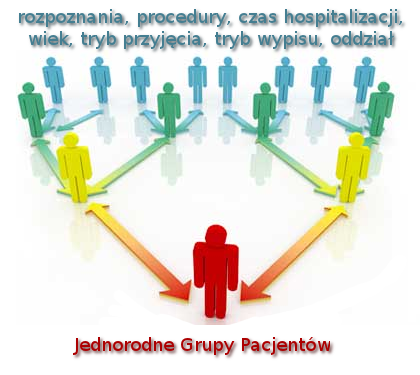
\includegraphics{images/standarization}

%---------------------------------------------------------------------------

\section{Historia systemu Jednorodnych Grup Pacjentów}
\label{sec:historiaJGP}

Początki systemu JGP sięgają lat 60-tych XX wieku systemu opieki zdrowotnej w USA. Wtedy zaobserwowano, iż pacjenci z tym samym schorzeniem, którym wykonywano te same badania i procedury oraz których czas hospitalizacji był zbliżony, generowali te same koszty. Na przełomie lat 60. i 70. prof. Robert Fetter z Uniwersytetu Yale po raz pierwszy przedstawił założenia systemu Jednorodnych Grup Pacjentów (Diagnosis Related Groups – DRG). Pacjenci podobni medycznie i kosztowo zostali przyporządkowani do 333 grup, w 54 głównych kategoriach diagnostycznych. Prof. Robert Fetter oparł się na analizie danych 1 mln 700 tys. pacjentów hospitalizowanych w szpitalach stanu New Jersey. Ostatecznie w Stanach Zjednoczonych system DRG wprowadzono w życie decyzją Kongresu w roku 1982.

Zaproponowany system zaczął się upowszechniać w Europie pod koniec lat 90. XX wieku. W Polsce pierwsze próby implantacji modelu DRG miały miejsce jeszcze w czasach Kas Chorych:
\begin{enumerate}
\item Grupy JGP w ginekologii i położnictwie w Łódzkiej Kasie Chorych w 1999 roku, opracowane na podstawie danych o kosztach leczenia pacjentek z 10 szpitali z województwa warmińsko-mazurskiego
\item Wdrożenie systemu JGP do rozliczeń świadczeń szpitalnych w Dolnośląskiej i Podkarpackiej Kasie Chorych w latach 1999 - 2003
\item Projekt adaptacji austriackiego systemu LKF zrealizowany w ramach projektu Banku Światowego w latach 2000 – 2002
\item Doświadczenia zebrane w trakcie trwania projektu VITAPOL komponent-3: „Przegląd polskiego systemu ustalania kosztów w opiece zdrowotnej” – umowa twinningowa realizowana przez brytyjskich ekspertów.
\end{enumerate} 
To właśnie brytyjski system HRG stał się podstawą opracowania polskiego modelu Jednorodnych Grup Pacjentów JGP. System Jednorodnych Grup Pacjentów w leczeniu szpitalnym został wprowadzony w Polsce 1 lipca 2008, a jego głównym twórcą jest dr Jacek Grabowski, ekspert systemów opieki zdrowotnej, z wykształcenia lekarz psychiatra.

W chwili obecnej system JGP jest zalecany przez Komisję Europejską na terenie całej Unii Europejskiej. Rozpoczęto prace nad projektem Euro-DRG 7, który docelowo stanowiłby jednolity system JGP dla całej Unii Europejskiej.


\chapter{Opis stworzonego rozwiązania}
\label{cha:rozwiazanie}

Niniejszy rozdział zawiera opis systemu, który został stworzony na potrzeby tej pracy. W rozdziale~\ref{sec:zalozeniaProjektowe} zostały krótko przedstawione najważniejsze założenia, na których opiera się realizacja projektu. Następnie rozdział~\ref{sec:architekturaSystemu} opisuje architekturę stworzonego rozwiązania. Rozdział~\ref{sec:modelDanych} zawiera szczegółowy opis w jaki sposób został określony model danych. Sposób działania algorytmu grupowania został zaprezentowany w rozdziale~\ref{sec:gruperNFZ}. Spojrzenie na system z punktu widzenia systemu ekspertowego został zawarty w sekcji~\ref{sec:systemEkspertowy}. Rozdział~\ref{sec:optymalizacjaJGP} przedstawia realizację maszyny wyjąśniającej, która jest narzędziem umożliwiającym przeprowadzenie optymalizacji JGP w systemie.
%Na końcu rozdział {sec:} opisuje szczegółowo przepływ danych oraz sterowania w systemie.

%---------------------------------------------------------------------------
%---------------------------------------------------------------------------
\section{Założenia projektowe}
\label{sec:zalozeniaProjektowe}

Na kształt aplikacji bezpośredni wpływ miały założenia projektowe postawione na początku pracy. Od nich zależały decyzje podejmowane na kolejnych etapach tworzenia systemu.

\begin{itemize}
 \item Swtorzyć aplikację typu ,,gruper'' spełniającą wszystkie wymagania stawiane przez NFZ.
 \item Określić model danych, ustalić bazę wiedzy.
 \item System zostanie napisany w języku JAVA, będzie to aplikacja desktopowa z dostępem do bazy wiedzy, zapisanej w jednym pliku.
 \item Zastosować architekturę warstwową dla systemu
 \item Użyć najnowszych i najlepszych narzędzi do tworzenia przyjaznego dla użytkownika GUI.
 \item Projekt architektury oprzeć na metodologii Spring.
 \item W trakcie fazy implementacji zwrócić szczególną uwagę na to, aby system spełniał założenia systemu ekspertowego. Implementacja systemu będzie zalążkiem do stworzenia bardziej rozbudowanego systemu ekspertowego dla tego rozwiązania.
 \item Używać tylko narzędzi dostępnych na licencji wolnego oprogramowania.
 \item Wykonać solidne testy dla wszystkich głównych ścieżek poszukiwań rozwiązania.
\end{itemize}

Stworzenie aplikacji typu ,,gruper'' oznacza, że musi zostać zaimplementowany algorytm grupera zgodnie z wytycznymi narzuconymi przez NFZ. Precyzyjne określelnie modelu danych jest podstawowym założeniem, bez którego niemożliwa jest dalsza praca na projektem. Zastosowanie architektury warstwowej dla systemu zwiększa elastyczność rozwiązania i pozwala na łatwe modyfikowanie i skalowalność systemu.

Implementacja całego systemu tylko w języku JAVA umożliwia rozwijanie projektu przez osoby nie znające składni oraz zasad jakimi kierują się inne języki dedykowane dla systemów ekspertowych takie jak Prolog czy Drools. Wszystkie założenia systemu ekspertowego zostają spełnione, ale implementacja będzie w 100\% autorska w czystej JAVIE. Fakty i reguły będą obiektami JAVY. Unikalność, innowacyjność i łatwość wdrożenia się w projekt dla tego rozwiązania mają być jego największymi atutami.



%---------------------------------------------------------------------------
%---------------------------------------------------------------------------
\section{Architektura systemu}
\label{sec:architekturaSystemu}

Wybór architektury systemu to decyzja podejmowana w początkowej fazie powstawania systemu. Często okazuję się ona najważniejszą decyzją, która ma ogromny wpływ na rozwój oprogramowania. Kierując się wyborem architektury, stawiałem na jej elastyczność oraz modularność. Obrazując system jako maszynę złożoną z wielu rożnorodnych elementów, chciałem stworzyć taką, którą można w łatwy sposób ulepszać poprzez dokładanie nowych oraz naprawiać poprzez podmianę starych części nowymi, lepszymi.

%---------------------------------------------------------------------------
\subsection{Model 3-warstwowy}
\label{sec:model3warstwowy}
Architektura systemu odzwierciedla jego logiczny podział. Standardem w praktycznie każdej aplikacji jest zastosowanie architektury trójwarstwowej. Jest to bardzo stara idea i sięga roku 1978. Kiedy to komitet ANSI/SPARC wprowadził podział na trzy warstwy:
\begin{itemize}
 \item Fizyczną implementację systemu
 \item Abstrakcyjny model wycinka rzeczywistości odzwierceidlany przez system
 \item Sposób w jaki jest postrzegany z zewnątrz - spojrzenie z punktu widzenia użytkownika końcowego
\end{itemize}

Jeżeli odniesiemy architekurę trójwarstwową do systemów informatycznych to odpowiednikiem schematu wewnętrznego jest warstwa bazy danych, schematu konceptualnego - warstwa biznesowa, a schematu zewnętrznego warstwa aplikacji. Architekturę przedstawia rysunek:
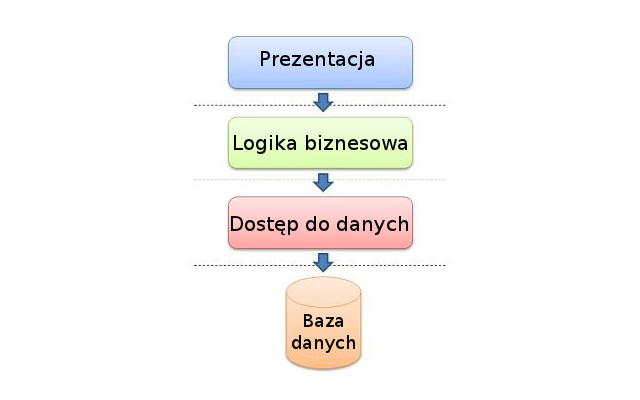
\includegraphics[scale=0.31]{images/3layer-architect}

Wybrałem ten model do zastosowania przy tworzeniu aplikacji ze względu na jego logiczną i zrozumiałą dla każdego informatyka modularność. Każda z warstw może zostać zaimplementowana w innym języku programowania, a łączą się one poprzez interfejsy. Dużym plusem tego rozwiązania jest łatwa możliwość zmiany pewnej części systemu bez zmian w innych częściach systemu. Dla przykładu, jeśli chcielibyśmy stworzyć GUI webowe to wystraczy tylko zaimplementować warstwę prezentacji i podpiąć się do warstwy logiki biznesowej.

%---------------------------------------------------------------------------
\subsection{Model architektury Spring}
\label{sec:modelArchitekturySpring}
Bardzo popularnym i nowoczesnym środowiskiem, które wprowadza zestaw narzędzi, wzorców oraz bibliotek potrzebnych do stworzenia nowoczesnych aplikacji serwerowych(i nie tylko) jest Springframework. Architektura Spring jest niesłusznie uważana za skomplikowaną, bardzo złożoną i niemożliwą do opanowania. W rzeczywistości architektura Spring stanowi zaawansowany przykład architektury szkieletowej umożliwiającej szybkie rozwijanie dowolnie złożonych aplikacji, niekoniecznie webowych. Konstrukcja szkieletu architektury Spring powoduje, że jest ona typem tzw. lekkiej infrastruktury, w której występuje bardzo niewielki stopień zależności od interfejsów Spring API. Architektura Spring obejmuje wszystkie warstwy aplikacji i podsuwa rozwiązania, które mogą być stosowane zarówno w warstwie prezentacji, jak i w warstwie integracji i warstwie danych. Architektura Spring jest rozwijana na licencji ,,open sourc'' od roku 2003 i od tego czasu zdobyła sobie dużą popularność i spore grono osób programujących. Poniższy rysunek ilustruje schemat architektury Spring:

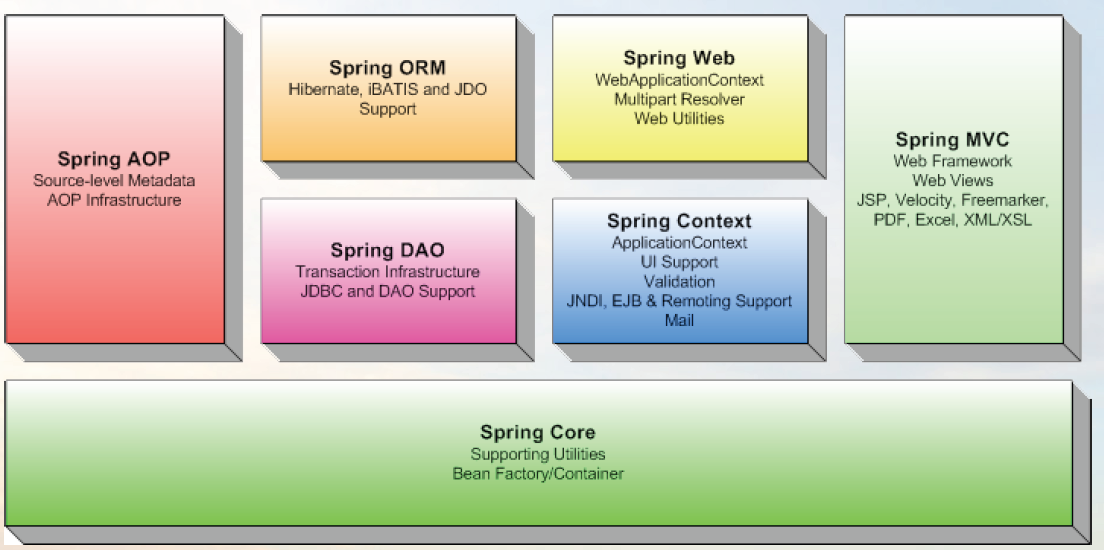
\includegraphics[scale=0.31]{images/spring-modules}

Architektura Spring składa się z kilku modułów, z których każdy może być wykorzystywany niezależnie w aplikacji. Oznacza to, że aplikacja może wykorzystywać całą moc architektury Spring, ale może także korzystać z fragmentu architektury, np. z modułu ułatwiającego dostęp do danych. Najważniejszym modułem architektury jest Spring Core, moduł oferujący zaawansowane opcje konfiguracji komponentów JavaBean oraz klas POJO(ang. Plain Old Java Object) i wykorzystujący technikę wstrzykiwania zależności.
Dla mojego rozwiązania postanowiłem skorzystać właśnie z tych dwóch fragmentów architektury Spring, tj dostęp do danych oraz Core dla warstwy serwisowej. Oto listing modułów Spring wykorzystywanych w projekcie:
\begin{itemize}
 \item JDBC - Java DataBase Connectivity - interfejs programowania opracowany w 1996 r. przez Sun Microsystems, umożliwiający niezależnym od platformy aplikacjom napisanym w języku Java porozumiewać się z bazami danych za pomocą języka SQL.
 \item DAO - Wzorzec projektowy Data Access Object (DAO) - rozdzielenie mechanizmu trwałości obiektów od reguł biznesowych
 \item Service - Spring Service Beans - obiekty serwisowe - wykonujące logikę biznesową
\end{itemize}

Dla warstwy prezentacji wykorzystałem również wsparcie Spring. W 2008 roku została wydana 1 wersja frameworku do tworzenia aplikacji desktopowych w JAVIE - SpringRCP - Rich Client Project. Niestety po wydaniu wersji 1.1 w 2009 projekt, który był na całkiem wysokim poziomie porównując do NetBeans-RCP lub Eclipse-RCP umarł śmiercią naturalną. W roku 2011 jeden z główynch projektantów Spring postanowił go odświeżyć. W niecałe 6 miesięcy przepisał cały framework używając najnowszej metodologii pochodzącej z Spring 3. Projekt ze względów politycznych musiał zmienić nazwę na Valkyrie-RCP. W kolejnych iteracjach dodanych zostało multum nowych funkcjonalności, w wyniku których po kolejnych 3 miesiącach powstało solidne narzedzie do tworzenia skomplikowanych aplikacji desktopowych w JAVIE. Jego podstawowe cechy to przejrzystość, prostota, stosowanie dobrych wzorców GUI. Kilka podstawowych elementów architektury Valkyrie:
\begin{itemize}
 \item Widget - komponent GUI (tabelka, forma, widok, edytor-danych)
 \item DataProvider - fasada danych dla komponentów UI.
\end{itemize}
Poniższy schemat przedstawia architekturę systemu jaki został zaimplementowany:

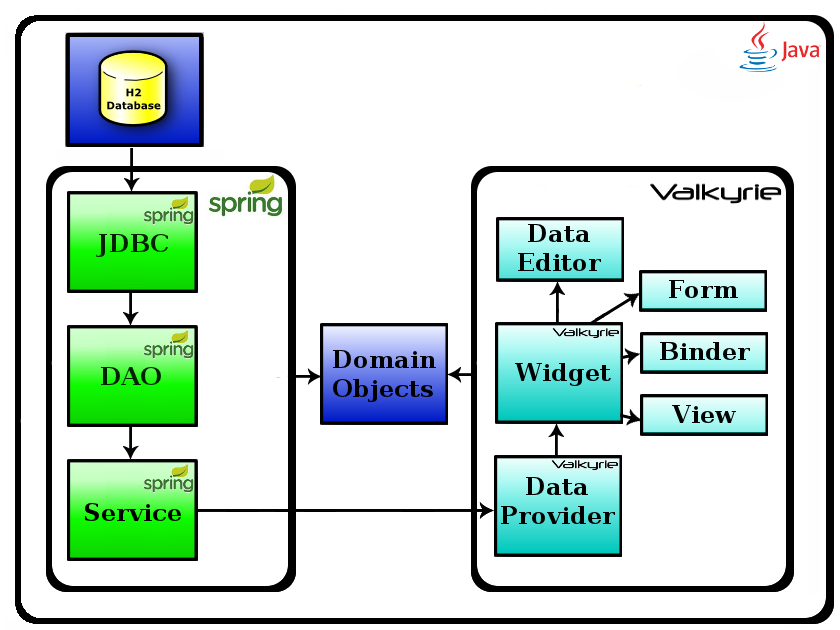
\includegraphics[scale=0.4]{images/spring-layers2}

Należy zaznaczyć, że model architektury spełnia założenia architekty trójwarstwowej:
\begin{table}[h]
 \caption{Moduły Spring jako elementy architektury trójwarstwowej}
 \small\tt
 \centering
 \vspace{0in}
 \begin{tabular}{|l|l|}
 \hline
 \textbf{3-warstwowa} & \textbf{Mój model} \\ 
 \hline
 Dostęp do danych & H2-Database, JDBC, DAO \\
 \hline
 Logika biznesowa & Services \\
 \hline
 Prezentacja & Valkyrie-RCP \\
 \hline
 \end{tabular}
\end{table}

%---------------------------------------------------------------------------
\subsection{Architektura systemu ekspertowego}
\label{sec:architekturaSystemuEkspertowego}
Jedna z definicji systemu ekspertowego definiuje go jako system charakteryzujący się strukturą:
\begin{itemize}
 \item Szkielet
       \begin{itemize}
	 \item Interfejs użytkownika
	 \item Edytor bazy wiedzy
	 \item Systemu wnioskujący
	 \item Mechanizm wyjaśniający
       \end{itemize}
 \item Baza wiedzy
 \item Danamiczna baza danych
\end{itemize}

Bardzo istotnym elementem systemu ekspertowego jest oddzielenie wiedzy dziedzinowej od reszty systemu. Takie podejście umożliwia usprawnienie działania systemu bez ingerencji w kod programu. W skrócie wyjaśnię elementy architektury systemu ekspertowego.

\textbf{Interfejs użytkownika} umożliwia zadawanie pytań, udzielanie informacji systemowi oraz odbieranie od systemu odpowiedzi i wyjaśnień.
\textbf{Edytor bazy wiedzy} pozwala na modyfikację wiedzy zawartej w systemie, umożliwiając tym samym jego rozbudowę.
\textbf{Mechanizm wnioskowania} jest głównym składnikiem systemu ekspertowego wykonującym cały proces rozumowania w trakcie rozwiązywania problemu postawionego przez użytkownika.
\textbf{Mechanizm wyjaśniający} jest to jeden z elementów interfejsu pomiędzy systemem a użytkownikiem, który umożliwia użytkownikowi uzyskanie odpowiedzi dlaczego system udzielił takiej, a nie innej odpowiedzi, albo dlaczego system zadał użytkownikowi określone pytanie.
\textbf{Baza wiedzy} jest to deklaratywna postać wiedzy ekspertów z danej dziedziny zapisana za pomocą wybranego sposobu reprezentacji wiedzy, najczęściej reguł.
\textbf{Danamiczna baza danych} jest pamięcią roboczą przechowującą pewne fakty wprowadzone w trakcie dialogu z użytkownikiem. Baza ta umożliwia odtworzenie sposobu wnioskowania systemu i przedstawienie go użytkownikowi za pomocą mechanizmu wyjaśniającego.
Architekturę systemu regułowego przedstawia poniższy schemat:
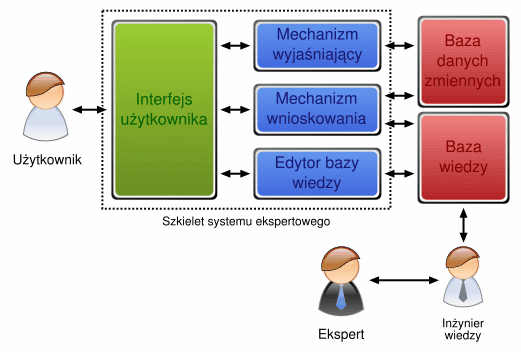
\includegraphics[scale=0.5]{images/expert-system}

%---------------------------------------------------------------------------
\subsection{System ekpertowy w architekturze Spring}
\label{sec:systemEkpertowyArchitekturaSpring}

Na początku pracy postawiona została teza: realizacja systemu ekspertowego w architekturze spring spełniającego wymagania dotyczące aplikacji grupera oraz zawierającego optymalizację grupowania.

Popularne narzędzia do implementacji systemu ekspertowego to język Prolog, system Drools, Jess, CLIPS. Są to gotowe środowiska do budowania skomplikowanych systemów ekspertowych. Dla tych systemów wystarczy zdefiniować wiedzę w postaci faktów i reguł, a następnie zadać cele, aby otrzymać wynik. Nie zdecydowałem się jednak na użycie tych dedykowanych systemów z dwóch ważnych powodów. Po pierwsze w mojej pracy postanowiłem zrobić coś innowacyjnego, a mianowice chciałem zbudować swój autorski system ekspertowy od podstaw zarazem używając do jego budowy nowoczesnych narzędzi. Stworzenie chociaż zalążka takiego innowacyjnego systemu w najnowszej technologii będzie już sporym osiągnięciem. Spojrzenie na system ekspertowy z naciskiem na jego realizację w czystej JAVIE może przynieść ciekawe rezultaty. 

Ten sposób myślenia doprowadził mnie do punktu, w którym musiałem jasno określić, które elementy systemu ekspertowego będą zaimplementowane przez które elementy architektury Spring. I tak określiłem, że warunki dla spełnienia reguł mogą być zapisywane jako obiekty POJO w bazie danych. Same reguły mogą być zapisywane w bazie poprzez sygnatury metod do wykonania lub jako skrypty napisane w języku Groovy(obiektowy język skryptowy wzorowany na składni Javy). Dynamiczna baza wiedzy będzie zrealizowana za pomocą obiektów POJO zapisywanych w bazie danych. Interfejs użytkownika  powstanie przy użyciu środowiska ValkyrieRCP, oraz jego wzorca DataEditor, który umożliwi dodawanie, edycję, usuwanie a nawet filtrowanie faktów oraz uruchamianie algorytmu wnioskowania. System wnioskujący będzie zrealizowany w warstwie biznesowej/serwisowej, gdzie zostanie zaimplementowany mechanizm wnioskowania. Będzie on wybierał dla danych wejściowych zestaw reguł i warunków, następnie wywoła metody sprawdzające i wykona odpowiednie działania jeśli warunki są spełnione. Mechanizm wyjaśniający zaimplementowany zostanie również w warstwie biznesowej.


%---------------------------------------------------------------------------
%---------------------------------------------------------------------------
\section{Model danych}
\label{sec:modelDanych}

W tym podrozdziale znajduje się opis w jaki sposób powstawał model danych dla aplikacji.

%---------------------------------------------------------------------------
\subsection{Dane wejściowe NFZ}
\label{sec:daneWejscioweNFZ}
Jedynym pewnym źródłem danych dla aplikacji były rozporządzenia NFZ. Fundusz opublikował ponad 30 wersji pliku parametryzującego, w formacie MS-Excel. W pliku parametryzującym znajdują się arkusze, w których zostały zapisane dane w postaci tabel zdefiniowanych przez NFZ. Każda następna wersja pliku parametruzyjącego przynosiła ze sobą zaktualizowane dane. Na przykład rozpoznania i procedury, które nie występowały w wersji wcześniejszej pliku parametryzującego. Z kolejnymi wydaniami wersji poprawiane zostały drobne błędy związane z formatem zapisu danych. Moją uwagę w trakcie porównywania wersji plików zwrócił zapis w kolumnie ranga procedury. Ranga większa niż 2 była zapisywana jako napis: '>2', co poprawiono na napis '3'. Ze względu na fakt, iż wiele poprawiono wraz z wydaniami kolejnych wersji pliku parametryzującego postanowiłem pracować na wersji 25, która jest jedną z najnowszych. 

Niestety nadal model danych pozostawiał wiele do życzenia. Na przykład w arkuszu o nazwie 'JPG' znajduje się listing wszystkich kodów JGP, jako kolumny przyjęte zostały wartości oddziałów - na przecięciu wiersza(kodu jgp, kodu produktu i nazwy jgp) i kolumny(oddział) postawiony został krzyżyk. W innym arkuszu dotyczącym wartości punktowej dla kodu JGP przepisane zostały jeszcze raz wszystkie kody jgp, kody produktu i nazwy jgp, a obok podane wartości punktowe. Kolejnym przykładem jest zdefiniowanie w arkuszu 'procedury' redundantnych danych - kody i nazwy procedur zduplikowane po 4-kroć, różniące się jedynie kolumną 'typ listy'.

Plik parametryzujący dostarczał redundantne dane, zduplikowane wartości w wielu tabelach, nieokreślone klucze podstawowe, obce, ograniczenia unikalności. Nasuwał się automatycznie jeden wniosek: model danych dostarczany przez NFZ musi koniecznie zostać przekonwertowany tak, aby nowy model danych zachowywał integralność. Konwersja bedzie polegała na zapimportowaniu danych z arkusza kalkulacyjnego do bazy danych, a następnie normalizacji bazy.

%---------------------------------------------------------------------------
\subsection{Relacyjna baza danych}
\label{sec:relacyjnaBazaDanych}

Postanowiłem wszystkie dane aplikacji przechowywać w relacyjnej bazie danych ze względu na nastepujące właściwości tego rozwiązania:
\begin{itemize}
 \item Wszystkie wartości danych oparte są na prostych typach danych.
 \item Wszystkie dane w bazie relacyjnej przedstawiane są w formie dwuwymiarowych tabel
 \item Po wprowadzeniu danych do bazy, możliwe jest porównywanie wartości z różnych kolumn, zazwyczaj również z różnych tabel, i scalanie wierszy, gdy pochodzące z nich wartości są zgodne. Umożliwia to wiązanie danych i wykonywanie stosunkowo złożonych operacji w granicach całej bazy danych.
 \item Wszystkie operacje wykonywane są w oparciu o algebrę relacji, bez względu na położenie wiersza tabeli.
 \item Z braku możliwości identyfikacji wiersza przez jego pozycję pojawia się potrzeba obecności jednej lub więcej kolumn niepowtarzalnych w granicach całej tabeli, pozwalających odnaleźć konkretny wiersz. Kolumny te określa się jako klucz podstawowy tabeli.
\end{itemize}
Uniwersalność tego rozwiązania pozwala zapisywać wszystkie typy danych, począwszy od typów prostych skończywszy na typach złożonych takich jak zserializowane obiekty JAVY, skrypty Groovy'iego lub pliki binarne. Według mnie takie podejście definiuje dużą elastyczność systemu. Na przykład planowana implementacja systemu ekspertowego będzie wymagała pewnego nakładu pracy projektowej i implementacyjnej szczególnie. Ale jestem przekonany, że rozwiązania tworzone pod konkretne problemy są lepiej zaprojektowane niż uniwersalne oraz najszybsze, co jest najważniejsze z punktu widzenia użytkownika końcowego.

Ważną decyzją jest również wybór silnika bazy danych. Ponieważ jednym z założeń projektowym było napisanie projektu w nowoczesnym języku programowania jakim jest JAVA postanowiłem wybrać silnik bazo-danowy napisany właśnie tylko i wyłącznie w czystej JAVIE. Szukałem również rozwiązania, które pozwoli mi na zapis/odczyt danych z pojedynczego pliku bez potrzeby instalacji całej machiny serwera w systemie operacyjnym. Skorzystałem z tabelki umieszczonej na stronie www.h2database.com:

\begin{table}[h]
 \caption{Porównanie właściwości}
 \tiny\tt
 \centering
 \vspace{0in}
 \begin{tabular}{|l|l|l|l|l|l|}
 \hline
  & \textbf{H2} & \textbf{Derby} & \textbf{HSQLDB} & \textbf{MySQL} & \textbf{PostgreSQL} \\
 \hline
 Pure Java & Yes & Yes & Yes & No & No \\
 \hline
 Memory Mode & Yes & Yes & Yes & No & No \\
 \hline
 Encrypted Database & Yes & Yes & Yes & No & No \\
 \hline
 ODBC Driver & Yes & No & No & Yes & Yes \\
 \hline
 Fulltext Search & Yes & No & No & Yes & Yes \\
 \hline
 Multi Version Concurrency & Yes & No & Yes & Yes & Yes \\
 \hline
 Footprint (jar/dll size) & ~1 MB & ~2 MB & ~1 MB & ~4 MB & ~6 MB \\
 \hline
 \end{tabular}
\end{table}

W końcu udało mi się znaleść silnik bazodanowy spełniający postawione przeze mnie wymagania. H2-database jest to rozwiązanie typu openSource, napisane w 100\% przez 1 osobę(Thomas'a Mueller'a). Zaletą silnika H2 jest jego innowacyjność. Autor stawia na łatwość użytkowania silnika bazy. Co objawia się bardzo łatwą konfiguracją, szybkim i prostym dostępem do administracji przez consolę H2, która jest uruchamiana w oknie przeglądarki. Brak potrzeby instalowania bazy danych w systemie operacyjnym jest kolejnym atutem tego rozwiązania. Funkcje importowania i eksportowania danych do/z plików zewnętrznych są wręcz intuicyjne. Dokumentacja do silnika jest przejrzysta spójna, cały czas na bieżąco aktualizowana. Chociaż rozwiązanie nie jest powszechnie znane, jednak tak duża firma jak Google stosuje go w niektórych swoich serwerowych rozwiązaniach.

%---------------------------------------------------------------------------
\subsection{Normalizacja danych}
\label{sec:normalizacjaDanych}

Dostarczony przez NFZ plik parametryzujący musi zostać poddany 'obróbce'. Każdy z arkuszy z pliku parametryzującego zapisałem w osobnym pliku CSV. Każdy z plików csv zaimportowalem(używając funkcji CSVREAD silnika H2) do osobnej tabeli tymczasowej.

\begin{lstlisting}[language=SQL]
CREATE TEMPORARY TABLE ICD9_TMP(
    LIST_CODE_ID VARCHAR(5) NOT NULL, -- Kod listy
    LIST_TYPE_ID CHAR(1) NOT NULL,    -- Typ listy
    CODE VARCHAR(7) NOT NULL,         -- Kod procedury ICD-9
    RANGE INT,                        -- Ranga procedury ICD-9
    NAME VARCHAR(255) NOT NULL        -- Nazwa procedury ICD-9
) AS SELECT LIST_CODE_ID, LIST_TYPE_ID, CODE, RANGE, NAME FROM CSVREAD('icd9.csv');
\end{lstlisting}

Po zaimportowaniu wszystkich tabel, następnym krokiem jest normalizacja bazy danych. Wprowadzenie kluczy publicznych i obcych, usunięcie zwielokrotnionych wierszy. Normalizaca według wykonywana była według 1PN, 2PN oraz 3PN. Kontynuując przykład z arkuszem 'icd9' napisałem skrypt SQL tworzący nowe tabele:

\begin{lstlisting}[language=SQL]
CREATE TABLE ICD_LIST_TYPE(
    ID CHAR(1) PRIMARY KEY,
    NAME VARCHAR(10) NOT NULL
);

CREATE TABLE ICD9(
    CODE VARCHAR(7) PRIMARY KEY,
    RANGE INT,
    NAME VARCHAR(255) NOT NULL
);

CREATE TABLE ICD9_LIST(
    CODE VARCHAR(5) PRIMARY KEY
);

CREATE TABLE ICD9_LIST_CODE(
    ICD9_CODE VARCHAR(7) NOT NULL,
    LIST_CODE VARCHAR(5) NOT NULL,
    LIST_TYPE CHAR(1) NOT NULL,
    PRIMARY KEY (ICD9_CODE, LIST_CODE),
    FOREIGN KEY(ICD9_CODE) REFERENCES ICD9(CODE),
    FOREIGN KEY(LIST_TYPE) REFERENCES ICD_LIST_TYPE(ID),
    FOREIGN KEY(LIST_CODE) REFERENCES ICD9_LIST(CODE)
);
\end{lstlisting}

Po utworzeniu poprawnego schematu danych importujemy dane z tabel tymczasowych:

\begin{lstlisting}[language=SQL]
INSERT INTO ICD_LIST_TYPE (ID, NAME) VALUES ('G', 'globalna');
INSERT INTO ICD_LIST_TYPE (ID, NAME) VALUES ('U', 'do sekcji');
INSERT INTO ICD_LIST_TYPE (ID, NAME) VALUES ('H', 'do grupy');
INSERT INTO ICD_LIST_TYPE (ID, NAME) VALUES ('N', 'negatywna');

INSERT INTO ICD9 (CODE, RANGE, NAME)
 SELECT DISTINCT CODE, RANGE, NAME FROM ICD9_TMP ORDER BY CODE;

INSERT INTO ICD9_LIST (CODE)
 SELECT DISTINCT LIST_CODE_ID FROM ICD9_TMP ORDER BY LIST_CODE_ID;

INSERT INTO ICD9_LIST_CODE (ICD9_CODE, LIST_CODE, LIST_TYPE)
 SELECT CODE, LIST_CODE_ID, LIST_TYPE_ID FROM ICD9_TMP ORDER BY CODE;
\end{lstlisting}

Postępując podobnie udało mi się przenieść wszystkie potrzebne dane z arkuszy kalkulacyjnych do tabel bazy danych SQL. Wprowadziłem relacje poprzez ustalenie kluczy publicznych oraz obcych. Dla kolumn wymagających wprowadzenia ograniczenia unikalności, zostało ono dodane. W miejscach gdzie spodziewałem się bardzo dużej ilości zapytań wyciągających dane po kolumnie wprowadziłem indeksację kolumny w celu szybszego działania instrukcji SELECT.
Wynikiem działania mojej pracy jest 16 plików SQL. Skrypty importują dane do tabel tymczasowych, następnie wykonują operacje tworzące tabele spełniając warunek spójności oraz zabiegające anomaliom bazo-danowym. Na samym końcu przepisujące dane. Skrypty zostały uporządkowane w kolejności, w której muszą zostać wykonane, aby stworzyć model bazy danych wypełniony danymi wejściowymi NFZ. Poniższy listing zawiera wszystkie wyróżnione tabele:

\begin{table}[h]
   \caption{Model danych}
   \tiny\tt
   \centering
   \vspace{0in}
   \begin{tabular}{|c|l|l|l|}
      \hline
      \textbf{arkusz} & \textbf{plik CSV} & \textbf{plik SQL} & \textbf{Nazwa tabeli} \\
      \hline
      wersja JGP & - & - & - \\
      \hline
      ograniczenie pobytu & - & 1\_time\_unit.sql & TIME\_UNIT \\
      \hline
      ograniczenie wieku & - & 2\_age\_limit.sql & AGE\_LIMIT \\
      \hline
      ograniczenie pobytu & - & 3\_hospital\_limit.sql & HOSPITAL\_LIMIT \\
      \hline
      JGP & jgp\_department.csv & 4\_department.sql & DEPARTMENT \\
      \hline
      ograniczenie trybu przyjęcia & - & 5\_income\_mode\_limit.sql & INCOME\_MODE\_LIMIT \\
      \hline
      ograniczenie trybu wypisu & - & 6\_outcome\_mode\_limit.sql & OUTCOME\_MODE\_LIMIT \\
      \hline
      - & - & 7\_patient.sql & PATIENT \\
      \hline
      wykaz specjalności komórek & specialization\_unit.csv & 8\_specialization\_unit.sql & SPECIALIZATION\_UNIT \\
      \hline
      wykaz specjalności komórek & specialization\_unit.csv & 8\_specialization\_unit.sql & SPECIALIZATION\_UNIT\_EXCLUDE\_SERVICE \\
      \hline
      listy procedur & icd9.csv & 9\_icd\_list\_type.sql & ICD\_LIST\_TYPE \\
      \hline
      listy procedur & icd9.csv & 10\_icd9.sql & ICD9 \\
      \hline
      listy procedur & icd9.csv & 10\_icd9.sql & ICD9\_LIST \\
      \hline
      listy procedur & icd9.csv & 10\_icd9.sql & ICD9\_LIST\_CODE \\
      \hline
      listy rozpoznań & icd10.csv & 11\_icd10.sql & ICD10 \\
      \hline
      listy rozpoznań & icd10.csv & 11\_icd10.sql & ICD10 \\
      \hline
      listy rozpoznań & icd10.csv & 11\_icd10.sql & ICD10\_LIST\_CODE \\
      \hline
      zakresy JGP & jgp.csv & 12\_jgp.sql & JGP \\
      \hline
      zakresy JGP & jgp.csv & 12\_jgp.sql & JGP\_POINT\_VALUE \\
      \hline
      mechanizm osobodni & jgp\_hospital.csv & 13\_jgp\_hospital.sql & JGP\_HOSPITAL \\
      \hline
      JGP & jgp\_department.csv & 14\_jgp\_department.sql & JGP\_DEPARTMENT \\
      \hline
      parametry JGP & jgp\_parameter.csv & 15\_jgp\_parameter.sql & JGP\_PARAMETER \\
      \hline
   \end{tabular}
\end{table}



%---------------------------------------------------------------------------
\newpage
\subsection{Diagram ERD}
\label{sec:diagramERD}

W wyniku dogłębnej analizy oraz procesu projektowania bazy danych poprzez normalizację danych z pliku parametryzującego powstał spójny model danych. Logiczną strukturę wynikowego modelu ilustruje diagram ERD(Entity Relationship Diagram):

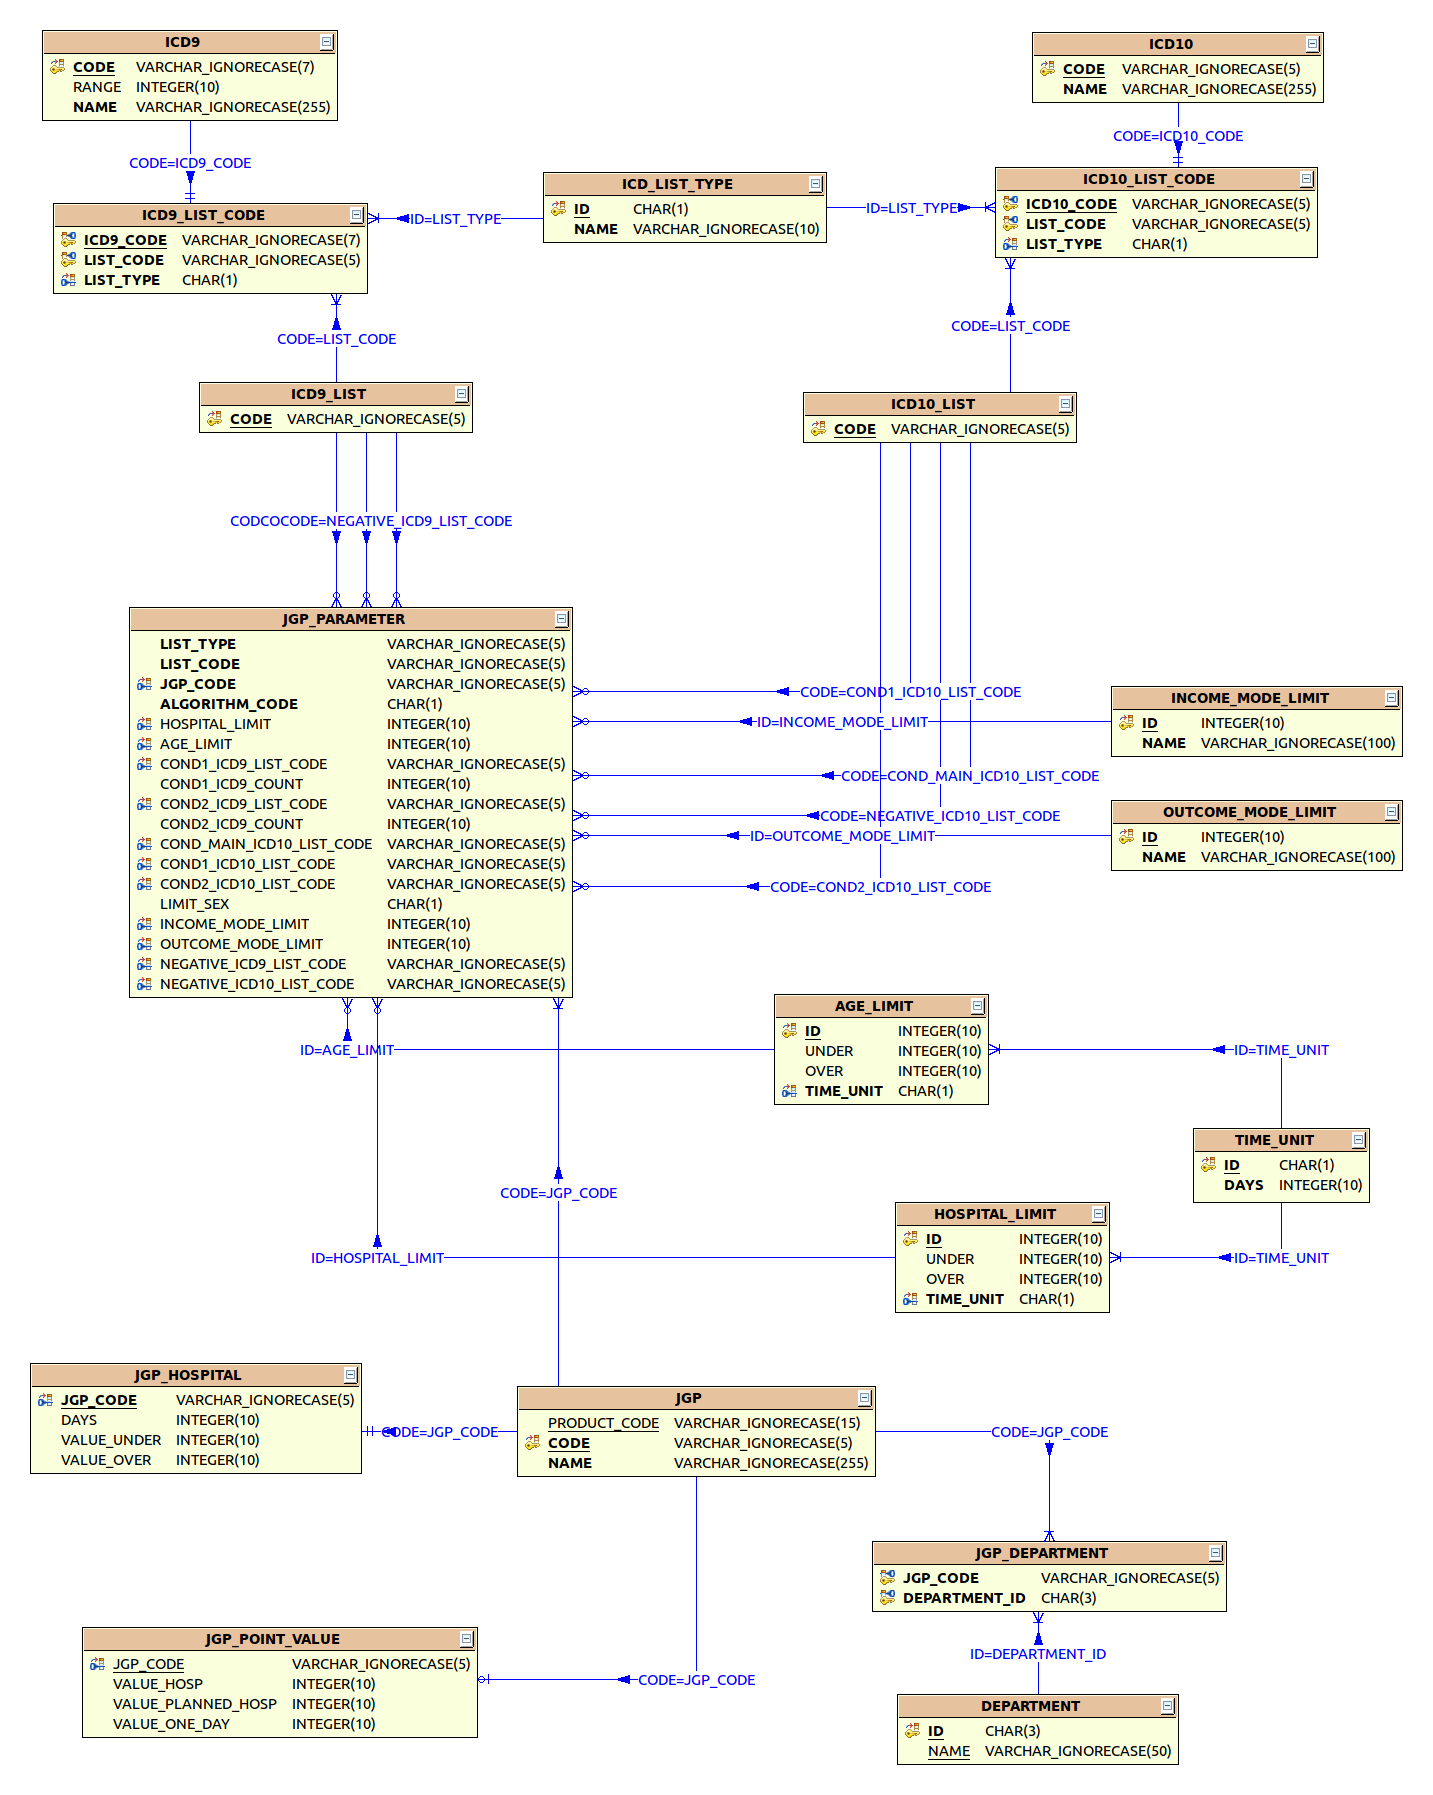
\includegraphics[scale=0.31]{images/erd}

%---------------------------------------------------------------------------
%---------------------------------------------------------------------------
\section{Gruper NFZ}
\label{sec:gruperNFZ}

W tym rozdziale znajduję się skrócony opis działania algorytmu grupera. Kompletny opis algorytmu grupera został przedstawiony w dokumencie opublikowanym przez NFZ zatytułowanym: "Informacje do przygotowania aplikacji grupera na potrzeby szpitalnych systemów informatycznych umożliwiającego kwalifikację rekordu pacjenta do właściwej grupy systemu Jednorodnych Grup Pacjentów". Dokument ten stał się podstawowym źródłem do stworzenia bazowej implementacji systemu. Dokument ten jest ponad 30-stronnicowym opisem, w jaki sposób powinna działać aplikacja gruper. Opis słowny algorytmu jak i schematy bloczkowe są dalekie do standardów takich jak język UML. Okazały się moim jedynym oraz kluczowym źródłem wiedzy o zasadach kierujących algorytmem. Rozpracowanie algorytmu grupera, poznananie i zrozumienie zasad jakimi się kieruje było kluczowym punktem mojej pracy.

%---------------------------------------------------------------------------
\subsection{Zasady i logika grupowania}
\label{sec:zasadyLogikaGrupowania}
Wynikiem działania algorytmu jest grupa JGP, która spełnia określony zestaw warunków. Zestaw grup JGP oraz warunków jest wyznaczany na podstawie danych wejściowych opisujących hospitalizację pacjetna. Alogorytm w uproszczeniu sprowadza się do wyznaczania grupy JGP. Po wyznaczeniu listy grup następuje badanie mechanizmem przeliczania, jeśli grupa kwalifikuje się do zmiany wartości zostaje ona zmieniona zgodnie z algorytmem mechanizmu przelcizania. Przedstawiony poniżej diagram aktywności przedstawia działanie algorytmu grupera:

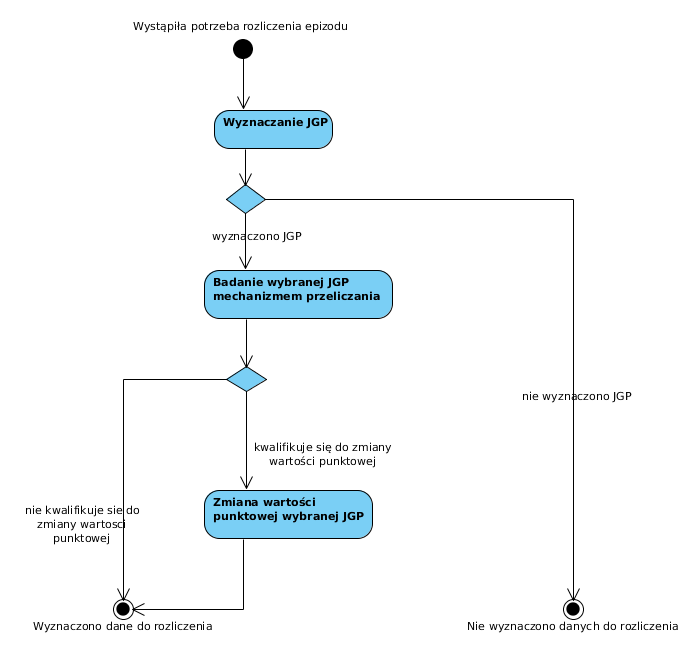
\includegraphics[scale=0.4]{images/activity-gruper}

%---------------------------------------------------------------------------
\subsection{Proces wyznaczania grupy systemu JGP}
\label{sec:procesWyznaczaniaGrupySystemuJGP}
Proces wyznaczania grupy można podzielić na dwie główne gałęzie. Pierwsza gałąź(tzw. ścieżka ICD-9) wyznacza zbiór zakwalifikowanych grup wraz z warunkami do sprawdzenia na podstawie procedur znaczących. Druga ścieżka 'ICD-10' wyznacza analogicznie zbiór zakwalifikowanych grup, ale na podstawie rozpoznań zasadniczych. Ścieżka dla rozpoznań jest wybierana przez program jeśli spełniony jest jeden z następujących warunków:
\begin{itemize}
\item w danych epizodu nie występuje żadna procedura
\item ranga procedury <= 2 i czas hospitalizacji > 1 dnia
\end{itemize}
Jeśli wymienione wyżej warunki nie są spełnione wybierana jest ścieżka ICD-9.

Następnie po wybraniu ścieżki wyznaczana jest lista kodów JGP wraz z warunkami do sprawdzenia. Każda grupa, która spełnia wszystkie warunki jest zapisywana na liście wybranych grup. Proces wyznaczania grupy dobrze ilustruje poniższy diagram aktywności:

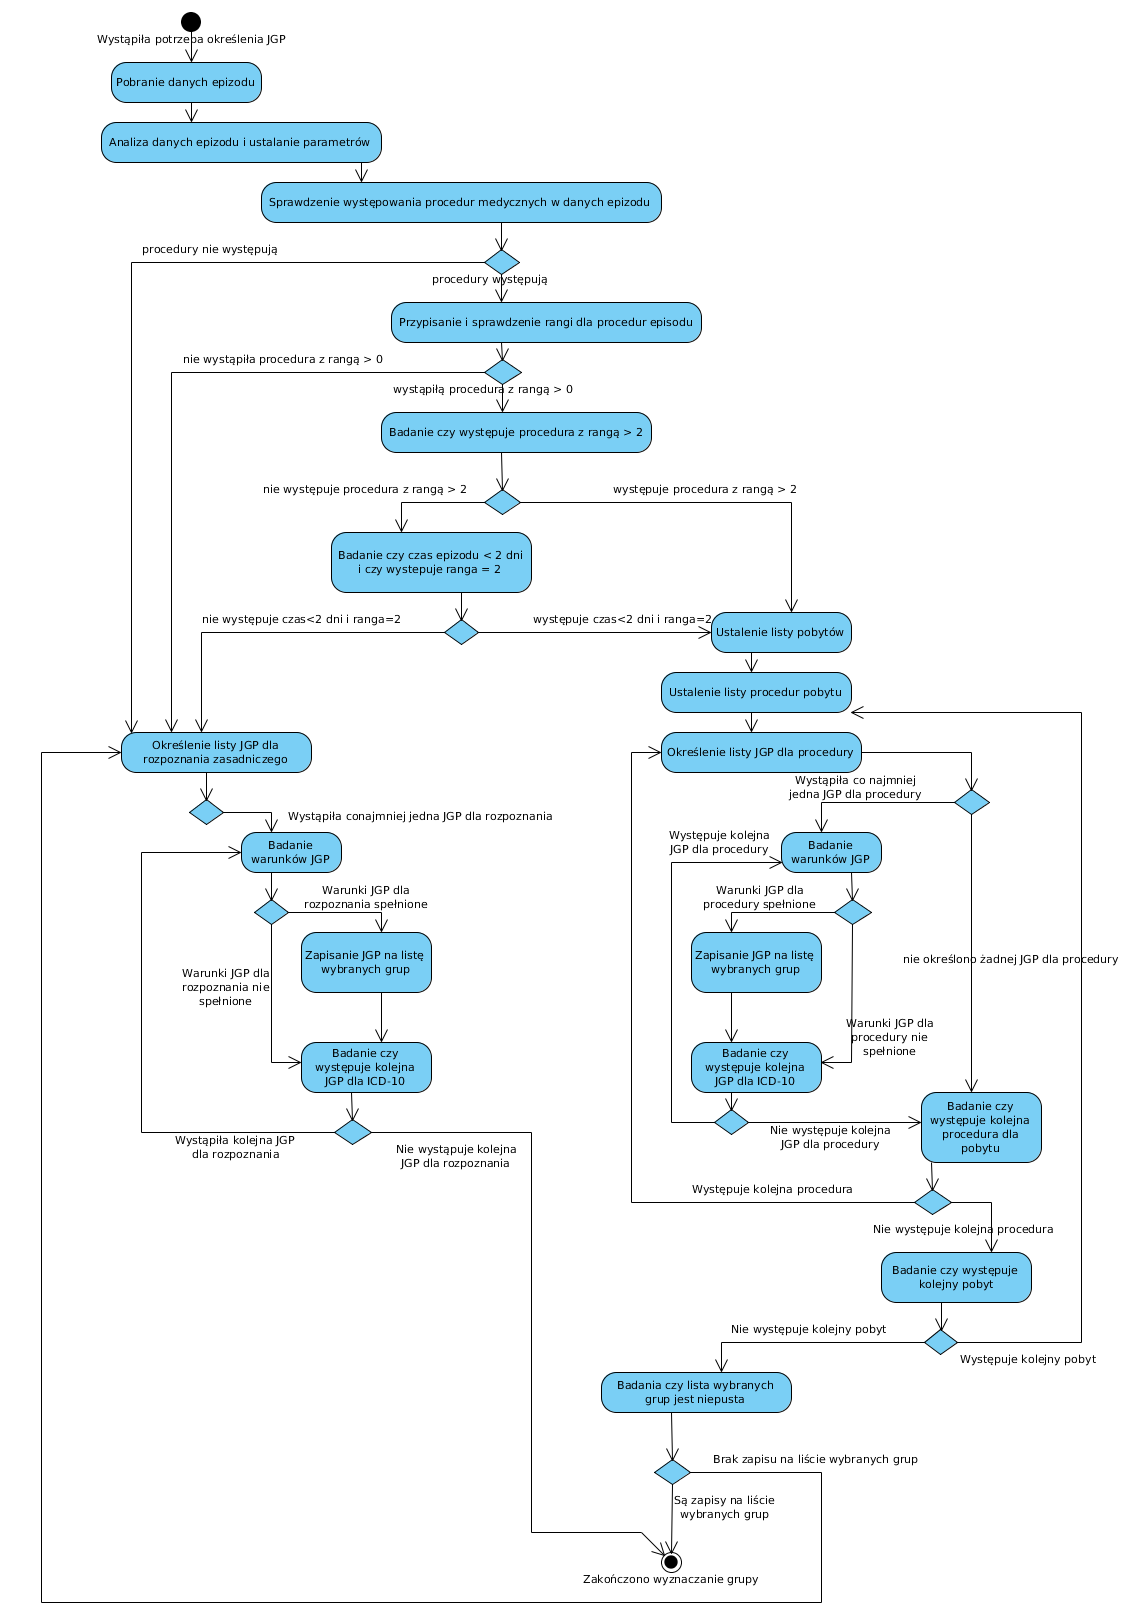
\includegraphics[scale=0.4]{images/activity-jgp} 

%---------------------------------------------------------------------------
\subsection{Warunki kierunkowe}
\label{sec:warunkiKierunkowe}
Warunki kierunkowe to decydujące o przebiegu grupowania ewentualne dodatkowe wymagania. Każdy z warunków został oznaczony literą alfabetu. A ich  dokładny opis znajduje się w dokumencie NFZ definiującym algorytm grupera. Procedura badająca warunki JGP w pierwszej kolejności sprawdza czy spełnione są warunki kierunkowe, ponieważ mają one decydujący wpływ na proces grupowania.
Sposób w jaki zdecydowałem się zaimplementować warunki kierunkowe:
\begin{itemize}
\item Każdy z warunków zapisany jest w bazie pojedynczą literą alfabetu (A-Z)
\item Dla obiektów domenowych literka alfabetu jest mapowana na odpowiednią wartość enuma Condition
\item zdefiniowanych jest 26 klas nazwanych dużymi literami alfabetu rozszerzających bazową klasę AbstractChecker oraz implementujących metodę:
  public abstract boolean checkCondition(Stay stay, JGPParameter parameter, List<Reason> reasons);
\item Utworzona została enum-mapa, w której kluczem jest enum(sygnatura warunku kierunkowego), a wartością obiekt(singleton) przypisanego do niej 'sprawdzacza' warunków
\end{itemize}
Zaletą tego podejścia jest możliwość implementacji w miarę uniwersalnego silnika do sprawdzania warunków kierunkowych. Działa on na zasadzie: dla każdego wybranego obiektu klasy JGPParameter(warunki które mają zostać sprawdzone) na podstawie odczytanej sygnatury warunku kierunkowego zostaje uruchamiany odpowiedni kawałek kodu JAVY sprawdzający warunki dla pobytu. A oto kawłek kodu realizujący tą funkcjonalność:

\begin{lstlisting}[language=Java]
private boolean checkDirectional(Stay stay, JGPParameter parameter, List<Reason> reasons) {
  //pobranie sygnatury(A-Z) warunku ktory powinien zostac sprawdzony
  Condition condition = parameter.getCondition();
  //pobranie checkera dla warunku z mapy
  AbstractChecker checker = conditionsMap.get(condition);
  Assert.notNull(checker, "not implemented checker for condition: " + condition);
  //uruchomienie odpowiedniego checkera i zwrocenie wyniku badania warunku
  return checker.checkCondition(stay, parameter, reasons);
}
\end{lstlisting}

W ten sposób udało mi się zapisać bardziej skomplikowane warunki w bazie danych. Tak naprawdę zapisana jest sygnatura checkera, a niestety dalej ważna część logiki jest zapisana w kodzie. Ale o rozszerzeniu tego rozwiązania  i zapisaniu całej logiki checkera do bazy danych napiszę więcej w rozdziale system ekspertowy.

%---------------------------------------------------------------------------
\subsection{Mechanizm osobodni}
\label{sec:mechanizmOsobodni}
Oczywistym faktem jest, że wyznacznikiem kosztów leczenia pacjenta nie może być tylko wartość wyliczona na podstawie przypisanej do pacjenta grupy systemu JGP. Ważnym czynnikiem generującym koszty leczenia jest czas pobytu w szpitalu(pożywienie, wymiana pościeli, podawane leki) wszystkie te koszty generowane są przez pacjenta w każdym dniu. Dlatego do algorytmu grupera wprowadzony został mechanizm osobodni. Przelicza on wyznaczoną wartość punktową w przypadku spełnienia pewnych warunków dla określonej grupy według określonych zasad. Na początku algorytm bada czy można zastosować mechanizm przeliczania:
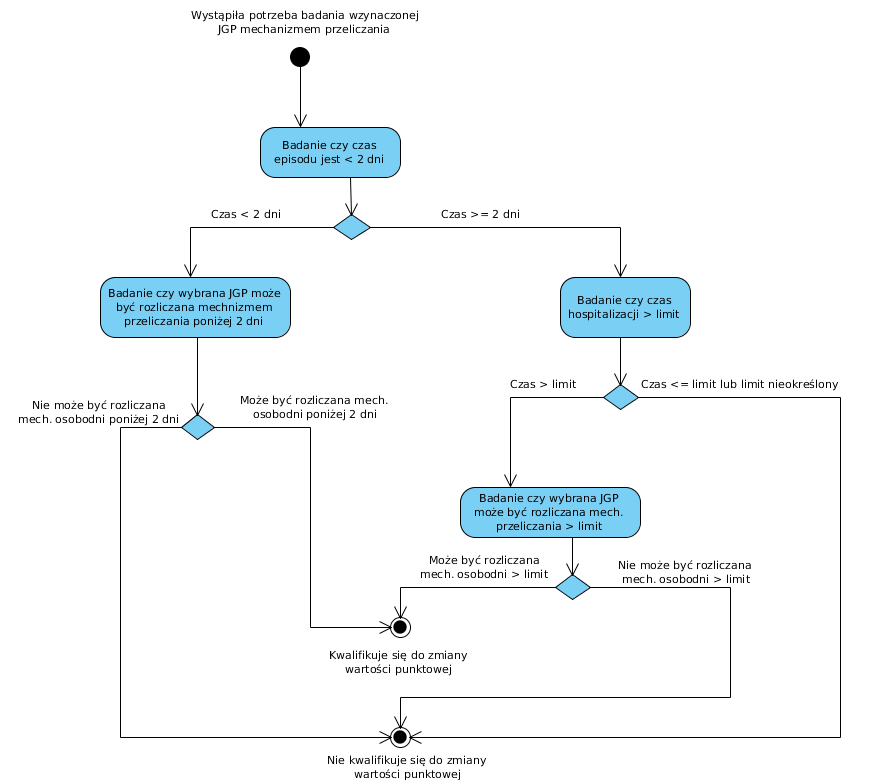
\includegraphics[scale=0.5]{images/activity-manday}

Jeśli wyznaczona grupa JGP dla epizodu nie kwalifikuje się do zmiany punktowej, pozostawiamy wartość wyznaczoną przez algorytm wyznaczania JGP. Natomiast jeśli zachodzi potrzeba zmiany punktowej stosujemy następujący algorytm dla 2 przypadków:
\begin{itemize}
\item Jeśli czas hospitalizacji jest mniejszy od 2 dni ustalamy nową wartość punktową ustalaną na podstawie wartości 'poniżej 2 dni' z obiektu klasy JGPHospital. Należy zaznaczyć, że z powyższego mechanizmu są wyłączone zgony, świadczenia rozliczane w ramach umów z zakresu ,,zespół opieki dziennej'' oraz ,,zespół chirurgii jednego dnia''.
\item Jeśli czas trwania episodu jest większy lub równy 2 dni i jest większy od limitu ustalonego na podstawie wartości ,,dni'' z obiektu klasy JGPHospital. To wartość JGP jest ustalana poprzez powiększenie aktualnej wartości JGP o wynik iloczynu dni powyżej limitu z wartością punktową określoną przez wartość "powyżej".

NOWA WARTOŚĆ PUNKTOWA = STARA WARTOŚĆ + RÓŻNICA DNI PONAD LIMIT * WAROŚĆ Z KOLUMNY POWYŻEJ
\end{itemize} 

%---------------------------------------------------------------------------
%---------------------------------------------------------------------------
\section{System ekspertowy}
\label{sec:systemEkspertowy}

Stworzenie systemu ekspertowego jest zadaniem bardzo trudnym. Postanowiłem, aby system który zaimplementowałem niejako dążył do systemu ekspertowego. Jest to tak zwane podejście ewolucyjne. To znaczy małymi kroczkami zbliżamy się w kierunku systemu ekspertowego, nie powstaje on od razu, ale w wyniku powolnej ewolucji, czyli przekszałceń pewnych części systemu. Pewne zmiany w implementacji sprawiają, że implementacja staje się coraz bardziej generyczna i uniwersalna. Zaletą takiego podejścia jest powolne, jasne i zrozumiałe wprowadzanie zmian w implementacji systemu, a co najważniejsze system ciągle spełnia stawiane mu wymgania. Wadą jest, że na efekt końcowy trzeba się sporo napracować.

\subsection{Klasyfikacja}
\label{sec:klasyfikacjaSystemuEkspertowego}
W tym podrozdziale chcę zakwalifikować system ekspertowy do odpowiednich klas systemów ekspertowych:
\begin{itemize}
 \item Ze względu na możliwość ingerencji człowieka w produkowane przez system rozwiązanie jest to tzw. system doradczy \textendash{} podpowiada rozwiązanie pomagając podjąć decyzję użytkownikowi \textendash{} prezentuje rozwiązanie jakiegoś problemu, ale do użytkownika należy jego ocena, oraz to czy je zaakceptuje, czy odrzuci.
 \item Ze względu na złożoność jest to system płytki - tzn. taki który korzysta tylko z informacji zgromadzonych w bazie wiedzy.
 \item Ze względu na dane otrzymywane na wyjściu jest to system:
   \begin{itemize}
    \item Diagnozy \textendash{} ocena istniejącego stanu na podstawie posiadanych danych
    \item Planowania \textendash{} opis stanu, do którego należy dążyć
   \end{itemize}
 \item Ze względu na rodzaj przetwarzanej informacji jest to system z wiedzą pewną.
\end{itemize}

\subsection{Baza wiedzy}
\label{sec:bazaWiedzy}
Najważniejszym z punktu widzenia systemu ekspertowego jest podział wiedzy na bazę faktów oraz bazę reguł. Logiczne wyróżnienie faktów dla systemu grupera JGP, pozwoli spojrzeć na system grupera jak na system ekpertowy. Wyróżnijmy więc fakty:
\begin{itemize}
 \item Rekord pacjenta
 \item Płeć
 \item Oddział
 \item Rozpoznanie(ICD-10)
 \item Procedura(ICD-9)
 \item Tryb przyjęcia
 \item Tryb wypisu
 \item Jednorodna Grupa Pacjentów
 \item Wartości punktowe dla JGP
 \item Czas hospitalizacji
\end{itemize}

oraz reguły:
\begin{itemize}
 \item warunki kierunkowe
 \item warunek na rozpoznanie główne
 \item warunek na rozpoznanie dodatkowe
 \item warunke na procedurę zasadniczą
 \item warunki na procedury dodakowe
 \item warunek na procedury i rozpoznania wykluczające się	
 \item ograniczenie na czas hospitalizacji
 \item ograniczenie na wiek
\end{itemize}
Spełnienie wyżej wymienionych warunków powoduje wykonanie akcji: zapisanie kodu JGP na listę kodów zaakceptowanych przez system. Model ten stosowany jest do wyznaczania grupy JGP.
Podobny mechanizm działa w trakcie wyznacznia nowych wartości mechanizmem osobodni.
Sprawdzane są warunki na czas hospitalizacji i jeśli są one spełnione wyznaczana jest nowa wartość punktowa.

\subsection{Maszyna wnioskująca}
\label{sec:maszynaWnioskujaca}
Realizacja maszyny wnioskującej w języku JAVA odbywa się przy użyciu Spring 3 na poziomie warstwy biznesowej. Klasa serwisowa przeprowadzająca proces wnioskowania zgodnie z wymaganiami systemu JGP to JGPService:

\begin{lstlisting}[language=Java]
public interface JGPService {
    public List<JGP> findJGP(final JGPFilter filter);

    public JGPGroupResult group(Episode episode);

    public JGPGroupResult doByProcedures(Episode episode);

    public JGPGroupResult doByRecognitions(Episode episode);

    public void resolveResultsByJGP(Stay stay, List<JGPParameter> parameters, JGPGroupResult jgpGroupResult);

    public void recountManDay(Episode episode, List<JGPResult> jgpResultList);

}
\end{lstlisting}

Metoda ,,group'' sprawdza którą ścieżkę wnioskowania obiera system - 2 opcje: wg. rozpoznania głównego lub wg. procedur zasadniczych. Metody ,,doByRecognitions'' oraz ,,doByProcedures'' wyznaczają zbiór warunków z charakterystyki JGP do przeanalizowania. metoda ,,resolveResultsByJGP'' wykonuje zasadnicze wnioskowanie:
\begin{itemize}\itemsep1pt
 \item Sprawdza warunki określone w obiekcie klasy JGPParameter i jeśli zostaną zaakceptowane zapisuje je na liście accepted.
 \item Metoda sprawdza warunki kierunkowe, warunek na płeć, warunek na tryb przyjęcia i wypisu, warunek na leczenie w danym oddziale, warunki na współisteniejące i zasadnicze kody ICD , warunki na kody ICD wykluczające się(negatywne).
\end{itemize}

Podusmowując maszyna wnioskująca dla poszukiwania optymalnej grupy JGP realizuje proces wnioskowania w następujących krokach. Przyjmuje zbiór faktów wejściowych w postaci obiektu klasy Episode. Następnie wybiera ścieżkę według, której mają zostać ustalone parametry JGP(ICD9 lub ICD10). Po ustaleniu ścieżki - wyciągane są z bazy reguły które mają zostać sprawdzone w postaci obiektu klasy JGPParameter. Następuje sprawdzenie warunków i w przypadku spełnienia wszystkich grupa zostaje zapisana na liście zaakceptowanych grup.


%---------------------------------------------------------------------------
%---------------------------------------------------------------------------
\section{Optymalizacja JGP}
\label{sec:optymalizacjaJGP}

W tym podrozdziale opisane zostanie zagadanienie optymalizacji kosztów leczenia pacjenta. W poprzednim podrozdziale ustaliliśmy, że maszyna wnioskująca wybiera zbiór parametrów do przetestowania. Następnie dla grup JGP spełniających warunki zapisuje je na liście ,,zaakceptowane''. W tym miejscu nasunęła się pewna myśl: A może by tak spróbować zapisać grupy JGP, które były testowane a odrzucone przez algorytm na listę grup niezaakceptowanych? Może dla każdej niezaakceptowanej grupy JGP obliczyć jaką wartość punktową mogłaby przyjąć gdyby była zaliczona. Oraz usprawnienie/ idea: dla każdej niezaakceptwanej grupy zapisać na liście powód -> dlaczego została ona niezaakceptowana - jakich warunków nie spełniła?

REALIZACJA: Aby zrealizować założenia, należało rozwinąć istniejący algorytm. Do obiektu klasy JGPResult dodałem listę niezaakceptowanych grup. Każda niezaakceptwana grupa będzie posiadać dodatkowo listę powodów niezaakceptowania - lista obiektów klasy Reason. W ten sposób, system będzie wiedział jakie warunki były testowane dla konkretnego rozwiązania oraz dlaczego nie zostały one zaakceptowane. 
Stworzyłem hierarchię klas dla powodów niezaakcpetowania:

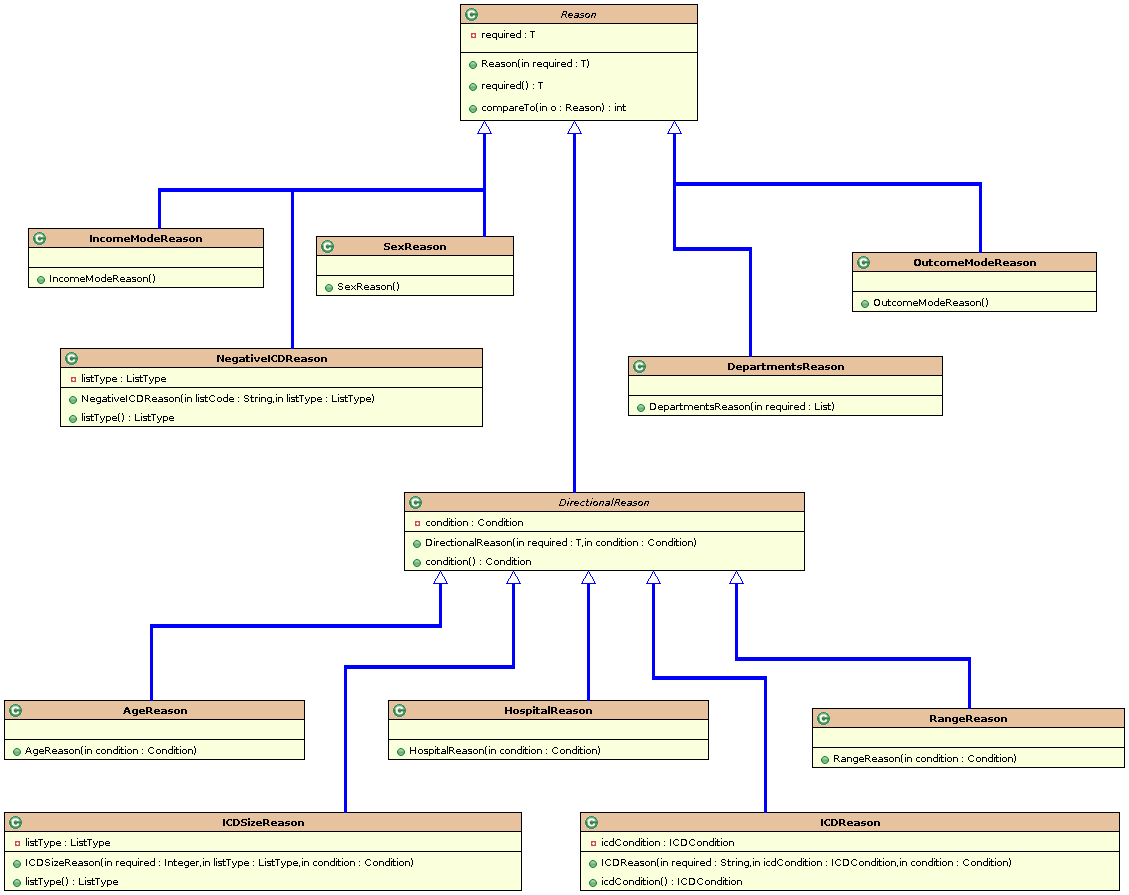
\includegraphics[scale=0.4]{images/reason-classes2}

Rozszerzyłem listę argumentów każdej z metod checkerów o argument: lista powodów niezaakceptowania: List<Reason> reasons. 
Po sprawdzeniu konkretnego warunku, w przypadku jego niezaakceptowania tworzona jest odpowiednia instancja obiektu Reason, a następnie jest ona  dodawana do listy. Np:

\begin{lstlisting}[language=Java]
protected boolean checkHospitalLimit(Stay stay, HospitalLimit hospLimit, List<Reason> reasons) {
     if (hospLimit != null) {
         int time = stay.getEpisode().hospitalTime(hospLimit.getTimeUnit());
         boolean result = hospLimit.test(time);
         if (!result) {
             reasons.add(new HospitalReason(hospLimit, condition()));
         }
         return result;
     }
     return true;
}
\end{lstlisting}

Np: Powodem niezaakceptowania grupy systemu JGP może być niespełnienie warunku: czas hospitalizacji dla grupy JGP musi być większy niż 7 dni, a zdefiniowany czas leczenia jest równy 5 dni.

Takie podejście pozwala na stworzenie funkocjonalności, która będzie podpowiadać lekarzowi jakie może uzyskać grupy JGP z większą wartości punktową, czyli jak zmaksymalizować koszty leczenia pacjenta. Program podpowiadałby również jakie konkretnie warunki musi spełnić hospitalizacja, aby zaliczyć ją do droższej grupy (wybranej przez lekarza).

Zaimplementowanie mechanizmu ,,Reasons - powody niezaakceptowania do grupy'' odpowiada w systemie ekspertowym modułowi objaśniająco-wyjąśniającemu(ang. Explanation Facility). Jest to część systemu odpowiedzialna za wyprowadzanie na zewnątrz wniosków systemu. Moduł ten daje użytkownikowi radę, sugestię, ale nie podejmuje decyzji. Zwróćmy uwagę, że zapis historii niespełnionych warunków pozwala odtworzyć część ścieżki poszukiwania rozwiązania dla rozwiązań niespełniających warunków.

\chapter{Prezentacja działania aplikacji}
\label{cha:prezentacja}

W tej części pracy znajduje się opis aplikacji widzianej oczami użytkownika. W rozdziale~\ref{sec:interfejsUzytkownika} został
przedstawiony interfejs graficzny użytkownika. Następnie rozdział~\ref{sec:praktyczneUzycieSystemu} prezentuje działanie aplikacji wykorzystując przykładowe dane hospitalizacji. W rozdziale tym znajduje się opis praktycznego użycia systemu dla realnych danych. Sekcja~\ref{sec:testyIntegracyjne} zawiera przykładowy test integracyjny jednej ze ścieżek poszukiwania rozwiązania.

%---------------------------------------------------------------------------

\section{Interfejs użytkownika}
\label{sec:interfejsUzytkownika}
Aplikacja posiada standardowo okienkowy interfejs użytkownika. Skórka aplikacji jest ustawiona na przyjazny ,,PlasticXPLookAndFeel''.

Wszystkie funkcjonalności, takie jak dodawanie, usuwanie, filtrowanie oraz cały widoczny układ komponentów graficznych dostarcza framework Valkyrie-RCP. Realizuje je klasa ,,DataEditor'', która jest komponentem graficznym(Widgetem). Do obiektu klasy ,,DataEditor'' wstrzykiwane są JavaBean'y: \textbf{DataProvider} - fasada danych dla interfejsu użytkownika, \textbf{DetailForm} - forma do dodawania/usuwania danych, \textbf{FilterForm} forma dla dodatkowego filtrowania oraz \textbf{TableWidget} - obiekt definiujący wyświetlaną tabelkę danych\cite{valkyrie_reference}.
Rysunek \ref{img:patient} ilutruje widok bazy pacjetnów, który jest oparty na szablonie ,,DataEditor''.

\begin{figure}[!ht]
\centering
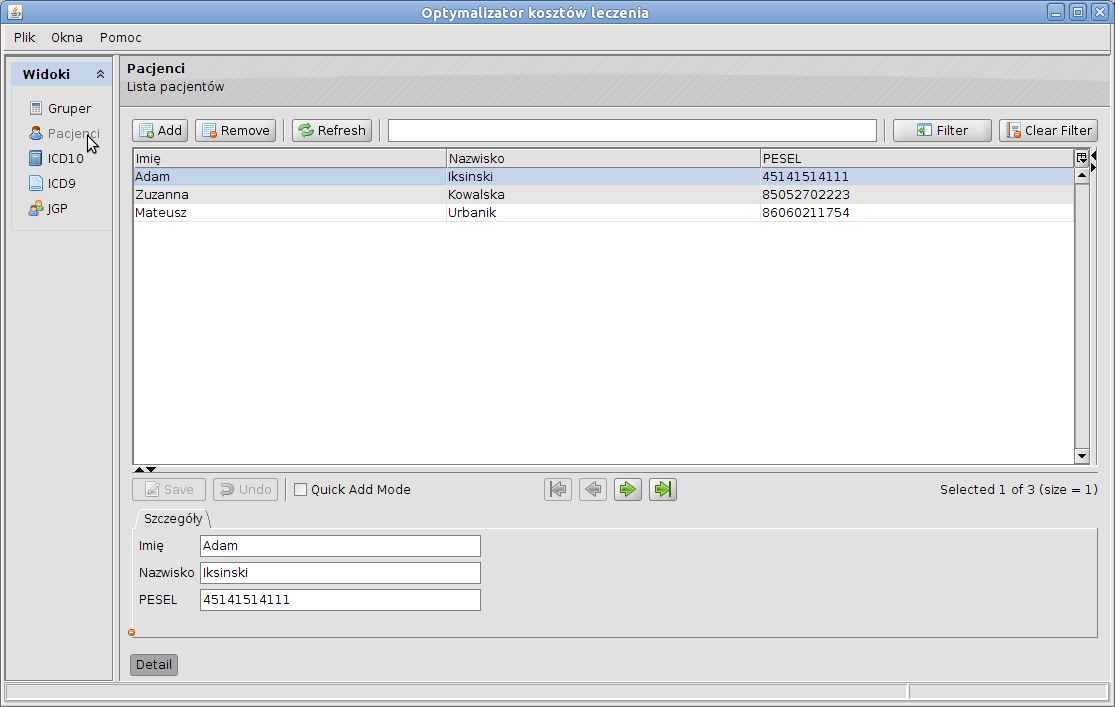
\includegraphics[scale=0.4]{images/patient} 
\caption[Widok bazy pacjentów]{Widok bazy pacjentów.}
\label{img:patient}
\end{figure}

W oparciu o wzorzec ,,DataEditor'' zbudowane są następujące widoki: katalog kodów \mbox{ICD-9}, \mbox{ICD-10}, JGP. Z tą różnicą w stosunku do widoku bazy pacjentów, że zablokowana jest dla nich możliwość dodawania, edycji i usuwania.

%---------------------------------------------------------------------------

\section{Praktyczne użycie systemu}
\label{sec:praktyczneUzycieSystemu}
Aby zilustrować działanie aplikacji przedstawiono w tym podrozdziale konkretny i realny przypadek użycia aplikacji. Zostanie wykorzystany również mechanizm dzięki, któremu lekarz ma możliwość optymalizacji kosztów leczenia pacjenta.

Zdefiniowano fakty wejściowe. Leczony pacjent urodzony w 1937 roku ma 75 lat, jest mężczyzną, przyjęty był na okres 7 dni w trybie przyjęcia ,,Przyjęcie planowe na podstawie skierowania'' oraz wypisany trybie ,,Zakończenie procesu terapeutycznego lub diagnostycznego''. Typ hospitalizacji ustalono na ,,Hospitalizacja zwykła''. Rysunek \ref{img:gruper1} przedstawia uzupełniony powyższymi danymi widok ,,Grupera''. 
Następnie należy zdefiniować pobyt. Do tego celu służy okno dialowe(Rys.~\ref{img:gruper2}) wyświetlane po kliknięciu przycisku ,,Dodaj pobyt''. Ustalono następujące dane pobytu: oddział, kod świadczenia. Data przyjęcia i wypisu przepisuje się automatycznie.
Kolejnym krokiem jest dodanie zdiagnozowanych rozpoznań(Rys.~\ref{img:gruper3}). Aby dodać rozpoznanie do pobytu należy kliknąć przycisk ,,Select''.
Następnie dodano wykonane procedury medyczne. W tym celu należy kliknąć przycisk ,,Dodaj procedurę''(Rys~\ref{img:gruper5}).
Po wybraniu procedury należy ustalić w jakim terminie została ona wykonana oraz ile razy(Rys.~\ref{img:gruper6}).
Zatwierdzenie przyciskiem ,,OK'' przenosi użytkownika do okienka z zdefiniowanym pobytem(Rys.~\ref{img:gruper7}).
Kiedy wszystkie dane dla pobytu zostały uzupełnione, zapis pobytu następuje po zatwierdzeniu przyciskiem OK(Rys.~\ref{img:gruper7}).
Widok ,,Gruper'' z wypełnionymi wszystkimi danymi wejściowymi prawidłowo pozwala użytkownikowi na uruchomienie algorytmu. Należy nacisnąć przycisk ,,Grupuj''(Rys.~\ref{img:gruper8}).

\begin{figure}%[!ht]
\centering
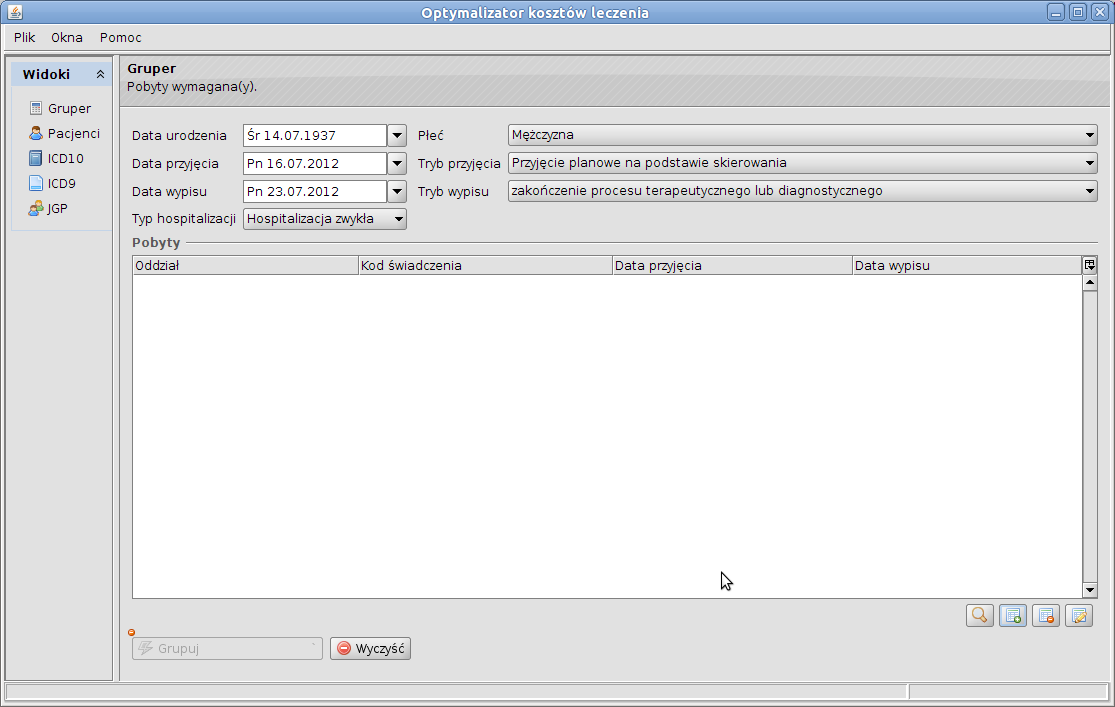
\includegraphics[scale=0.4]{images/gruper1}
\caption[Widok grupera]{Widok grupera - dane wejściowe.}
\label{img:gruper1}
\end{figure}

\begin{figure}%[!ht]
\centering
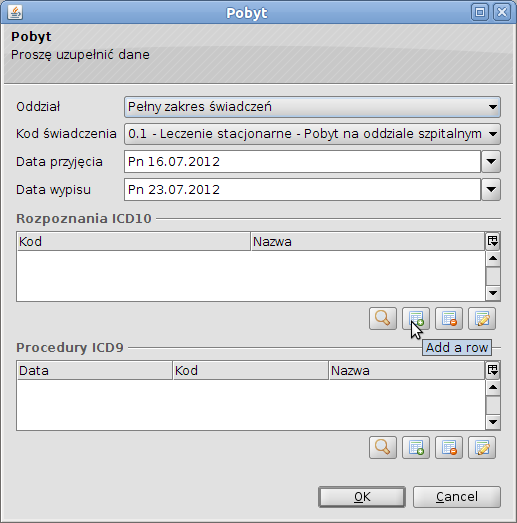
\includegraphics[scale=0.4]{images/gruper2}
\caption[Widok grupera]{Okno dialogowe - dodawanie pobytu.}
\label{img:gruper2}
\end{figure}

\begin{figure}%[!ht]
\centering
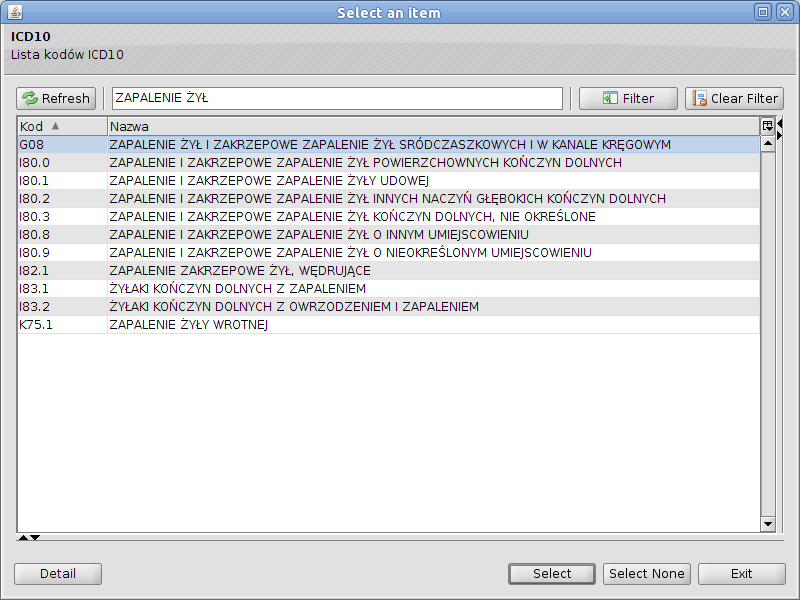
\includegraphics[scale=0.4]{images/gruper3}
\caption[Widok grupera]{Okno dialogowe - wybór rozpoznania.}
\label{img:gruper3}
\end{figure}

\begin{figure}%[!ht]
\centering
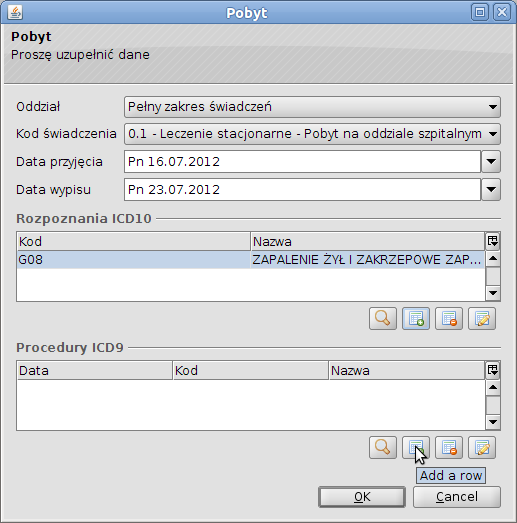
\includegraphics[scale=0.4]{images/gruper4}
\caption[Widok grupera]{Okno dialogowe - dodawanie pobytu - rozpoznanie.}
\label{img:gruper4}
\end{figure}

\begin{figure}%[!ht]
\centering
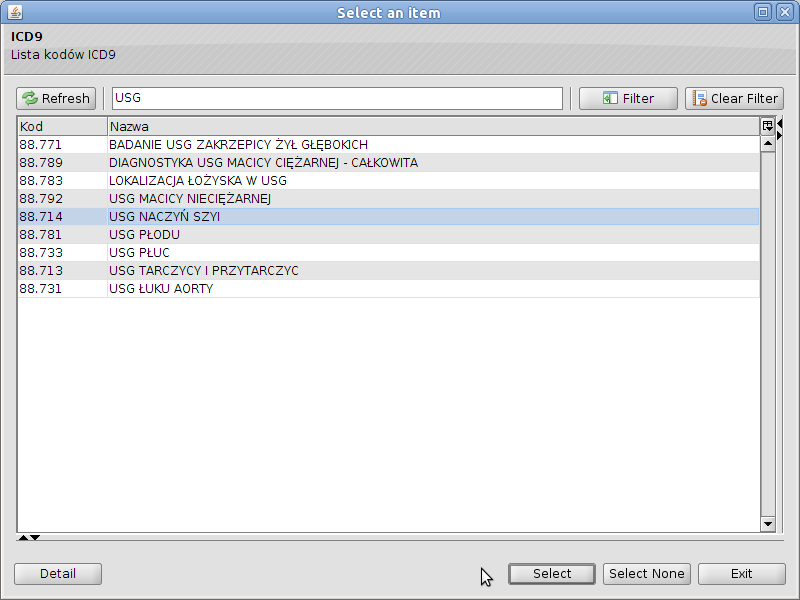
\includegraphics[scale=0.4]{images/gruper5}
\caption[Widok grupera]{Okno dialogowe - wybór procedury.}
\label{img:gruper5}
\end{figure}

\begin{figure}%[!ht]
\centering
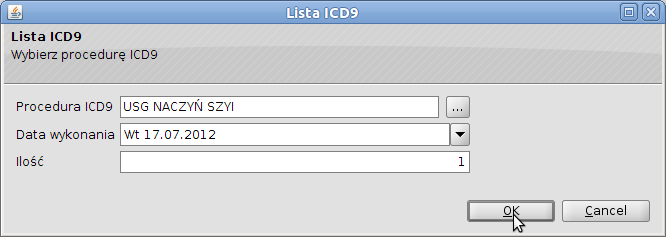
\includegraphics[scale=0.4]{images/gruper6}
\caption[Widok grupera]{Okno dialogowe - wybór procedury - data wykonania, ilość.}
\label{img:gruper6}
\end{figure}

\begin{figure}%[!ht]
\centering
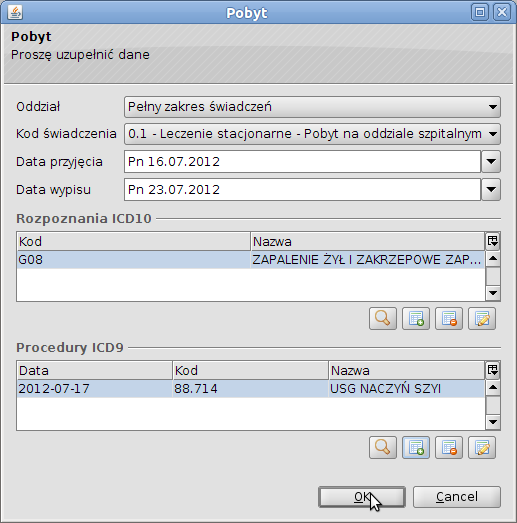
\includegraphics[scale=0.4]{images/gruper7}
\caption[Widok grupera]{Okno dialogowe - dodawanie pobytu - uzupełnione procedury i rozpoznania.}
\label{img:gruper7}
\end{figure}

\begin{figure}%[!ht]
\centering
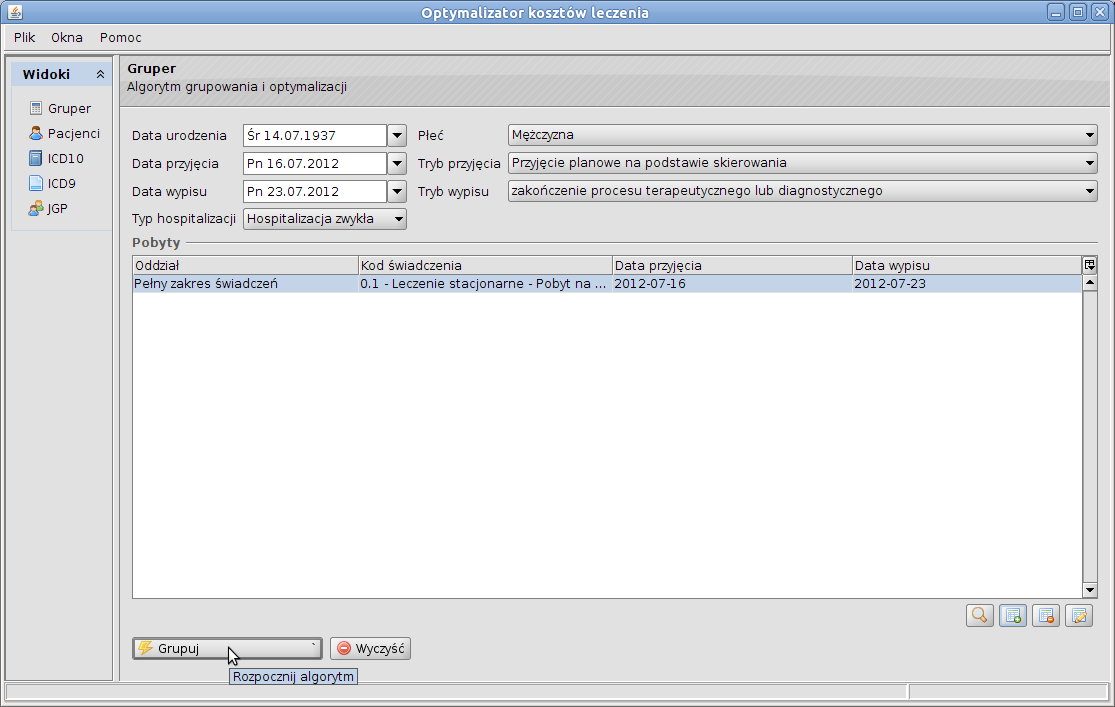
\includegraphics[scale=0.4]{images/gruper8}
\caption[Widok grupera]{Okno dialogowe - dodawanie pobytu - rozpoznanie.}
\label{img:gruper8}
\end{figure}

\begin{figure}%[!ht]
\centering
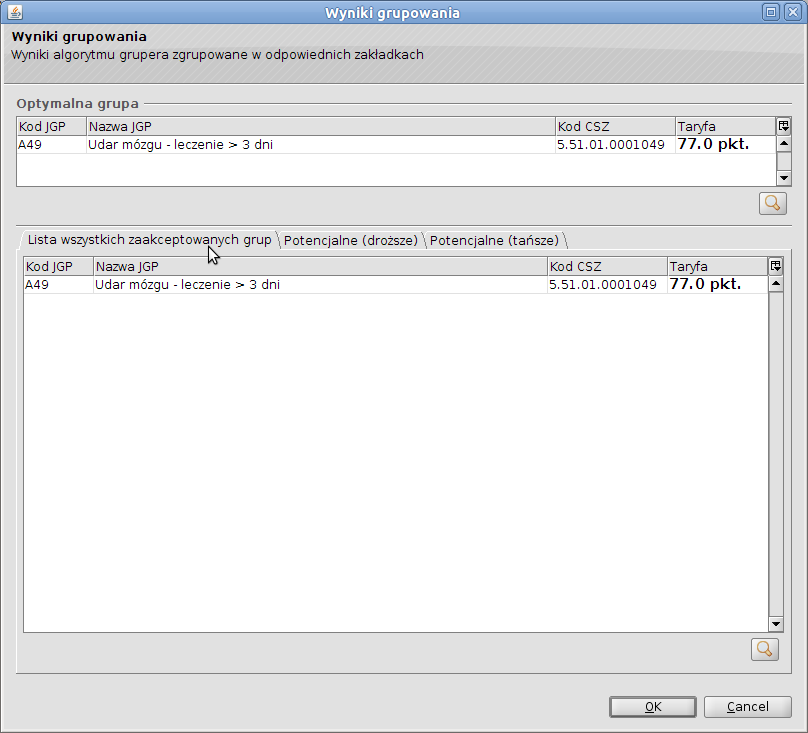
\includegraphics[scale=0.4]{images/gruper9}
\caption[Widok grupera]{Wyniki grupowania - Lista wszystkich zaakceptowanych grup.}
\label{img:gruper9}
\end{figure}

Uruchamiany jest algorytm wnioskowania, który wybiera warunki do sprawdzenia, testuje je, a~wyniki zapisuje na listach: Zaakceptowane, Potencjalnie droższe, Potencjalnie tańsze. W tym miejscu można zakończyć przebieg grupowania. Została wybrana optymalna grupa JGP: ,,A49 - Udar mózgu - leczenie > 3 dni'' oraz ustalona została wartość kosztów leczenia 77pkt(Rys.~\ref{img:gruper9}).

Następny krok w prezentacji działania aplikacji to optymalizacja kosztów leczenia. Przedstawione zostanie narzędzie pozwalające przewidywać wyliczane według NFZ koszty leczenia pacjenta. Przeprowadzony zostanie proces maksymalizacji kosztów leczenia. Na tym etapie należy spojrzeć na zakładkę ,,Potencjalnie droższe''(Rys.~\ref{img:gruper10}). Znajdują się tu grupy JGP, wśród których poszukiwane jest najlepsze rozwiązanie.

\begin{figure}%[!ht]
\centering
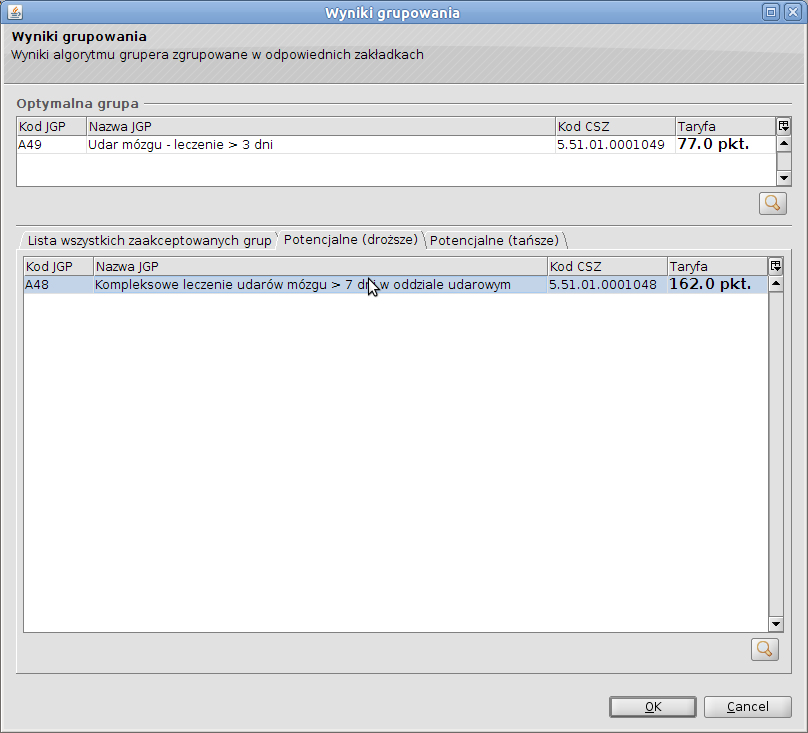
\includegraphics[scale=0.4]{images/gruper10}
\caption[Widok grupera]{Wyniki grupowania - Potencjalne (droższe).}
\label{img:gruper10}
\end{figure}

Zauważono, że istnieje grupa JGP dająca możliwość wygenerwoania kosztów w wysokości 162pkt. Jest to ponad dwukrotnie większa wartość od wyliczonej aktualnie. Należy kliknąć przycisk ,,Szczegóły'' i sprawdzić powody niezaakceptowania grupy A48(Rys.~\ref{img:gruper11}).

\begin{figure}%[!ht]
\centering
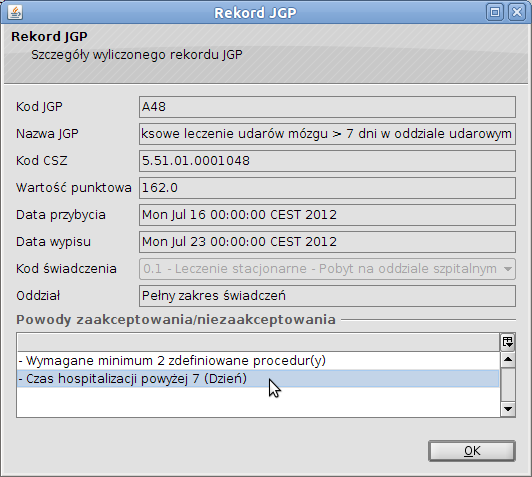
\includegraphics[scale=0.4]{images/gruper11}
\caption[Widok grupera]{Szczegóły niezaakceptowania grupy JGP.}
\label{img:gruper11}
\end{figure}

Z rysunku \ref{img:gruper11} można odczytać następujące powody niezaakceptowania pacjenta:
\begin{itemize}
 \item Wymagane jest zdefiniowanie 2 procedur medycznych,
 \item Wymagany jest czas hospitalizacji powyżej 7 dni.
\end{itemize}

W tym momencie zakres działania aplikacji się kończy. Jest to system doradczy, a decyzję optymalizacyjną podejmuje lekarz. Dla przedstawionego przypadku leczenia lekarz stwierdza, że przedłużenie pobytu na oddziale pacjenta o 1 dzień i wykonanie dodatkowego badania podwoi koszty leczenia. W tym przypadku lekarz może podjąć decyzję o przedłużeniu leczenia o 1 dzień(Rys.~\ref{img:gruper12}).

\begin{figure}%[!ht]
\centering
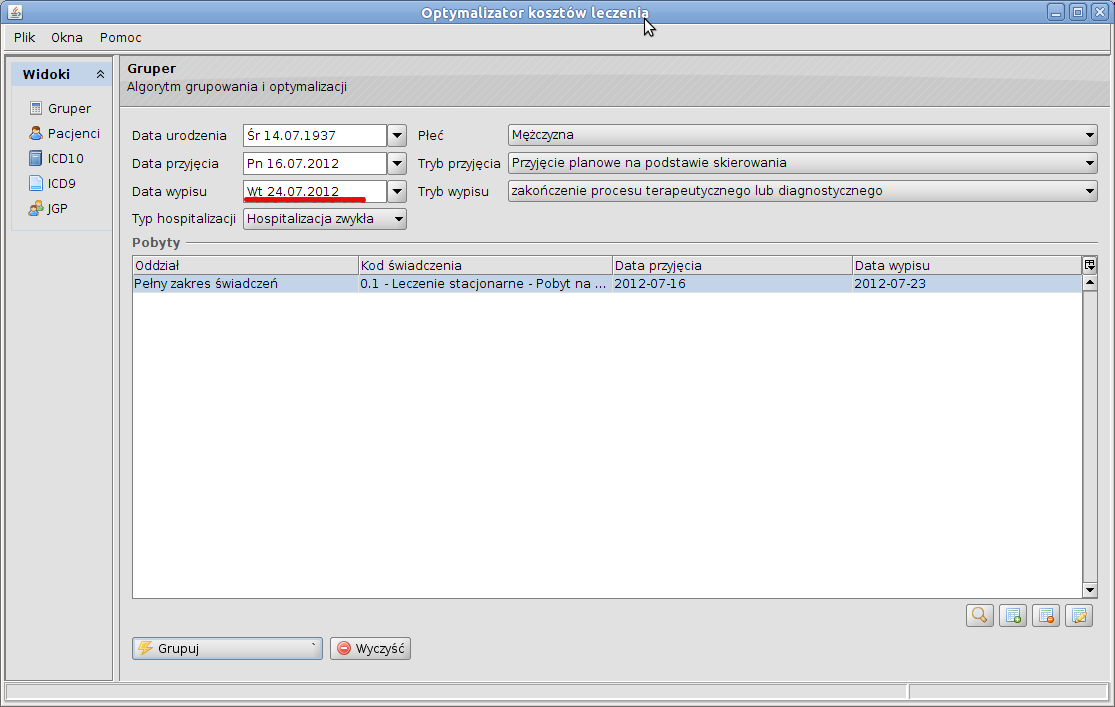
\includegraphics[scale=0.4]{images/gruper12}
\caption[Widok grupera]{Widok grupera - poprawione dane wejściowe.}
\label{img:gruper12}
\end{figure}

Dodano kolejną procedurę medyczną, badanie radiologiczne: ,,Arteriografia tętnicy szyjnej wewnętrznej''(Rys.~\ref{img:gruper13}, Rys.~\ref{img:gruper14}).

\begin{figure}%[!ht]
\centering
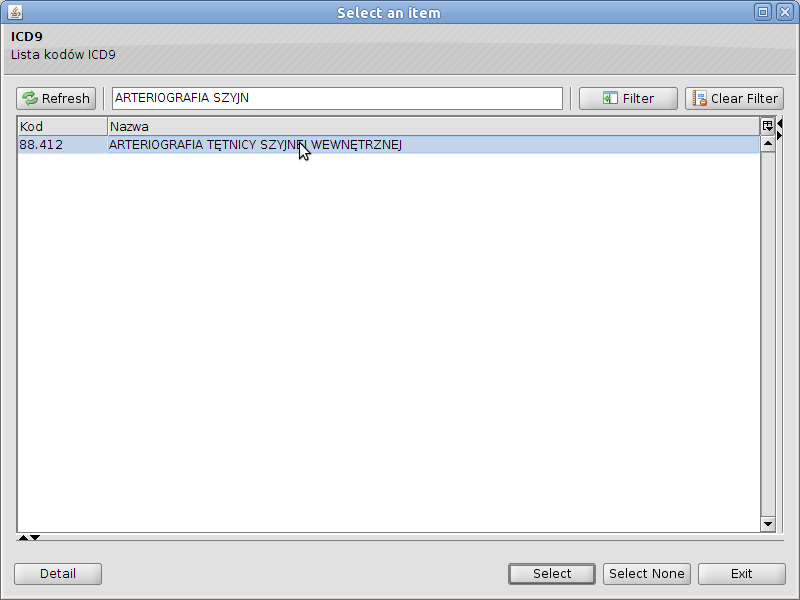
\includegraphics[scale=0.4]{images/gruper13}
\caption[Widok grupera]{Okno dialogowe - dodawanie procedury.}
\label{img:gruper13}
\end{figure}

\begin{figure}[!ht]
\centering
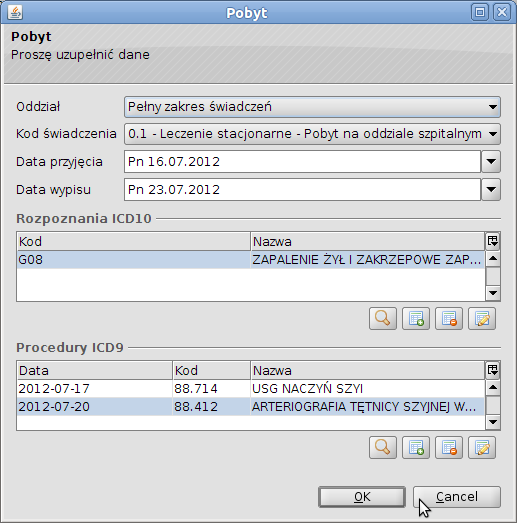
\includegraphics[scale=0.4]{images/gruper14}
\caption[Widok grupera]{Okno dialogowe - dodawanie pobytu - dodatkowo procedura.}
\label{img:gruper14}
\end{figure}

W wyniku ponownego uruchomienia algorytmu grupowania, otrzymano jako wynik spodziewaną grupę JGP(Rys.~\ref{img:gruper15}).

\begin{figure}%[!ht]
\centering
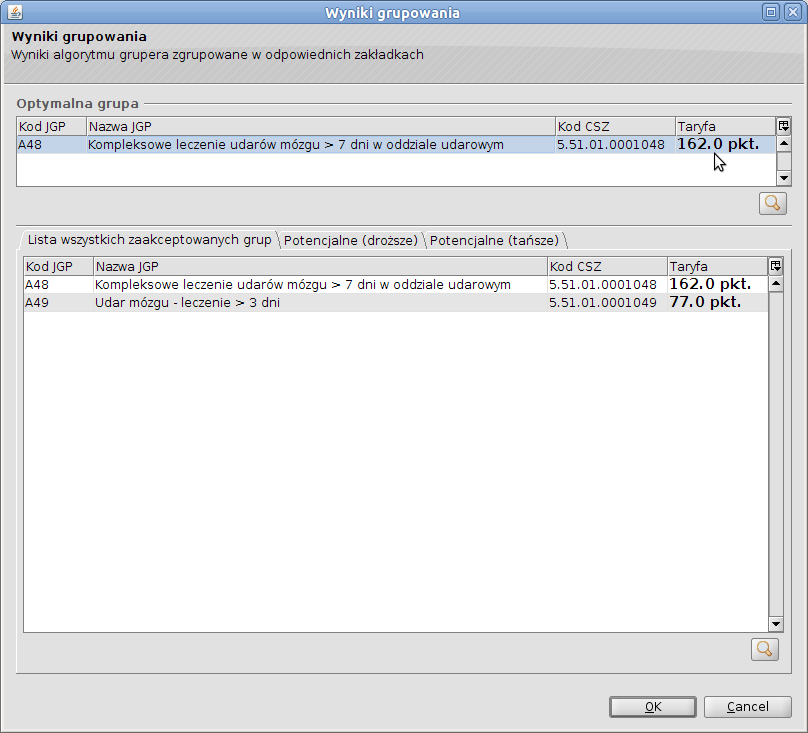
\includegraphics[scale=0.4]{images/gruper15}
\caption[Widok grupera]{Wyniki grupowania - Lista wszystkich zaakceptowanych grup.}
\label{img:gruper15}
\end{figure}

Wybrana zostaje grupa ,,A48 - Kompleksowe leczenie udarów mózgu > 7 dni w oddziale udarowym''. Zoptymalizowany koszt leczenia to 162 jednostki punktowe.

%---------------------------------------------------------------------------

\section{Testy integracyjne}
\label{sec:testyIntegracyjne}

Dobrą praktyką zwiększającą współczynnik jakości oprogramowania jest wysokie pokrycie kodu w testach. Zdecydowano się zatem napisać testy integracyjne klasy JGPService. Stworzono klasę ,,JGPServiceTest'', której zadaniem jest przetestowanie wszystkich głównych ścieżek algorytmu grupowania, gdzie testowana grupa wynikowa będzie pochodzić z konkretnego warunku kierunkowego. Zatem poszczególne testy są napisane w ten sposób, aby przetestować każdy z możliwych 26 warunków kierunkowcyh A-Z.
Przykład przedstawiony w sekcji \ref{sec:praktyczneUzycieSystemu} został również zaimplementwoany w testach. Test ten sprawdza poprawne działanie systemu dla warunku kierunkowego E - ,,grupa zdefiniowana procedurą i rozpoznaniem zasadniczym; może mieć dodatkowe warunki (czas hospitalizacji, wiek)''.
Dla testów integracyjnych przygotowana została testowa baza wiedzy. Przebieg testu jest następujący: ustalane są dane epizodu, uruchamiany jest mechanizm wnioskowania. Następnie sprawdzane są wyniki. Testowana jest poprawność wyników z listy zaakceptowanych kodów oraz z listy niezaakceptowanych kodów, wraz z testami zgodności powodów niezaakceptowania z wartościami oczekiwanymi.
Kod przykładowego testu integracyjnego zawiera listing \ref{java_test}.

\newpage
\begin{lstlisting}[language=Java,caption={Test integracyjny sprawdzający warunek kierunkowy ,,E''.},label=java_test]
@Test
public void testGrouperE() {
    Episode episode = createTestEpisode(new String[]{"G08"}, new String[]{"88.714"}, 7, 75);
    //run grouper
    JGPGroupResult result = jgpService.group(episode);
    //test accepted
    Assert.assertEquals(1, result.accepted().size());
    JGPResult acceptedJGP = result.accepted().get(0);
    Assert.assertEquals(77.0, acceptedJGP.getValue(), 0.0);
    Assert.assertEquals("A49", acceptedJGP.getJgp().getCode());
    //test NOT accepted
    Assert.assertEquals(1, result.notAccepted().size());
    JGPResult notAcceptedJGP = result.notAccepted().get(0);
    Assert.assertEquals(162.0, notAcceptedJGP.getValue(), 0.0);
    Assert.assertEquals("A48", notAcceptedJGP.getJgp().getCode());
    HospitalReason hospReason = notAcceptedJGP.reasons(HospitalReason.class).get(0);
    Assert.assertEquals(7, hospReason.required().getOver().intValue());
    Assert.assertEquals(TimeUnit.DAY, hospReason.required().getTimeUnit());
}
\end{lstlisting}


\chapter{Podsumowanie i wnioski}
\label{cha:podsumowanie}

Celem niniejszej pracy było stworzenie aplikacji ,,Gruper'' zgodnie ze specyfikacją NFZ. Aplikacja została zaprojektowana w ten sposób, aby spełniała założenia systemu ekspertowego. Następnie została rozszerzona tak, aby wspomóc proces optymalizacji kosztów leczenia pacjetna. Zadanie wymagało zdobycia i zrozumienia wiedzy z zakresu medycznegeo. Dostosowanie systemu tak, aby spełniał założenia systemu ekspertowego wymagało również odpowiedniego podejścia, ponieważ powinien on działać nie naruszając specyfikacji zdefiniowanej przez NFZ.

System, który stworzono jest zgodny z wszystkimi stawianymi na początku założeniami projektowymi. Jest on zalążkiem systemu ekspertowego, ponieważ inżynier może definiować reguły tylko w wydzielonym obszarze. W sekcji~\ref{sec:mozliwoscRozwoju} opisana została wizja możliwosci rozwoju systemu.

%---------------------------------------------------------------------------

\section{Możliwość rozwoju}
\label{sec:mozliwoscRozwoju}

Ze wględu na fakt, że aplikacja została napisana w modelu architektury warstowej, bardzo dobrym rozwinięciem istniejącego rozwiązania byłoby uruchomienie części odpowiadającej za logikę biznesową i za dostęp do danych na serwerze aplikacyjnym. Warstwę prezentacji można zaimplementować jako aplikację webową. Rozszerzenie to pozwala stworzyć system on-line z algorytmem ,,Grupera''.

Duże możliwości rozwoju projektu sprawia fakt, że jest to jedyne rozwiązanie typu ,,open source'' na rynku. Tego typu otwarte projekty przyciągają zainteresowanie jednostek, dla których rozwiązanie to jest dedykowane. Uruchomienie systemu do zgłaszania błędów i tworzenia własnych propozycji nowych funkcjonalności jest dobrym krokiem w kierunku rozwoju oprogramowania typu ,,open source''. Programiści, projektanci oraz architekci systemów z branży medycznej mogliby mieć własny wpływ na dalszy rozwój aplikacji.

Aplikacje zewnętrzne mogłyby korzystać z serwerowej części systemu. Takie rozwiązanie wspomaga proces tworzenia oprogramowania medycznego, ściągając z aplikacji do osługi szpitala odpowiedzialność za tworzenie własnej implementacji algorytmu ,,Grupera''. Warto zaznaczyć w tym miejscu, że jeśli lekarz nie posiada dedykowanej aplikacji ,,Grupera'' to jego obowiązkiem jest wyznaczanie grup JGP na podstawie arkusza MS-Excel opublikowanego przez NFZ\cite{plik_parametryzujacy}. 
Zakładając, że istniałby ogólnodostępny moduł do obsługi rozliczeń kosztów leczenia pacjenta, mógłby on być używany przez większość istniejących aplikacji. Rozwiązania komercyjne musiałyby jedynie połączyć się z modułem używając zewnętrznych serwisów. Projektanci, architekci i programiści mieliby dostęp do pełnej dokumentacji tego modułu i mogliby go w pełni wykorzystywać, nie tracąc cennego czasu na implmentację algorytmu od zera.

Ważnym kierunkiem rozwoju aplikacji byłby rozwój w kierunku systemu ekspertowego. Standaryzacja wiedzy, łatwość modyfikowania faktów i reguł systemu sprawiają, że jest on potężnym narzędziem w rękach ekspertów. Częste wprowadzanie zmian w regułach grupowania sprawia, że w standardowym podejściu, programiści muszą wprowadzać zmiany do kodu algorytmu. W podejściu ekspertowym zmiany te mogliby wprowadzać bezpośrednio inżynierowie wiedzy, bez potrzeby ingerencji w kod systemu.
%Pracownicy NFZ produkujący dokumentację w formie MS-Word(algorytm i reguły) i w MS-Excel bazę wiedzy, mogliby po zapoznaniu się z systemem używać go do tworzenia reguł w dedykowanym do tego języku.
%Wprowadzaliby oni dane do systemu jako inżynierowie wiedzy. Dodawaliby nowe fakty takie jak procedury, rozpoznania, kody jgp. Edytowaliby reguły, zmieniając warunki akceptacji grupy JGP, modyfikując obiekty klasy JGPParameters oraz powiązane z nimi obiekty klasy np. Agelimit, HospitalLimit. 
%Wszystkie warunki dla reguł mogliby edytować z poziomu dostępu ,,experta'' do systemu.
W takim podejściu zaleca się wyróżnienie dwóch ról: eksperta i użytkownia. Ekspert miałby dostęp do edycji faktów i reguł, a użytkownik do uruchomienia algorytmu wnioskowania.

Następną ścieżką rozwoju oprogramowania jest modernizacja jądra systemu ekspertowego, którym jest mechanizm wnioskowania. Aktualne rozwiązanie zapisuje warunki kierunkowe w bazie jako literki alfabetu. Krokiem w kierunku zapisywania pełnych reguł w systemie byłoby zapisywanie skryptów języka Groovy w bazie wiedzy, oraz udostępnienie ich do edycji dla użytkowników z rolą eskperta. Każdy z tych skryptów byłby pobierany i uruchomiany przez silnik w odpowiednim momencie.
%Dalszym rozwinięciem byłoby umieszczenie kolejnych skryptów Groovy w bazie wiedzy, które byłyby również uruchamiane przez silnik wnioskowania. Skryptem zapisanym w języku Groovy mogłaby być część kodu wybierająca odpowiednią ścieżkę poszukiwania(ICD9 lub ICD10) lub kod wyliczający wartości dla mechanizmu osobodni. 
Takie podejście tworzy uniwersalny system regułowy, którego algorytm mógłby być edytowany bez ingerencji w kod źródłowy programu.
%Inżynierowie wiedzy, jeśli nie pracownicy NFZ, to lekarze zainteresowani systemem wprowadzaliby poprawki w kluczowych dla algorytmu wycinkach kodu zapisanych w Groovy'm, ktory jest językiem bardzo czytelnym, przejrzystym, łatwym do nauczenia i zrozumienia dla każdego. W ten sposób otrzymalibyśmy spójny system ekspertowy usprawniający wszystkie aplikacje medyczne w Polsce z bazą wiedzy kontrolowaną przez NFZ, którego zadaniem byłoby wprowadzanie na bieżąco poprawek do algorytmu. Każda zewnętrzna aplikacja mogłaby podpiąc się do dedykowanych serwerów i używać grupowania zgodnego z zasadami NFZ.

Kolejnym pomysłem na rozwinięcie aplikacji jest używanie programowania aspektowego do zapisywania powodów niezaakceptowania warunku.
%Dla metod sprawdzających warunki można zrealizować zapisywanie powodów niezaakceptowania automatycznie poprzez aspekty, nie ręcznie jak dotychczas. 
Dla każdego sprawdzanego warunku byłaby zapisywana pełna lista powodów zaakceptowania lub niezaakceptowania.
Takie rozwiązanie dałoby całościowy obraz scieżki wyszukiwania dla wszystkich sprawdzanych rozwiązań.

Wydanych zostało ponad 10 wersji algorymtu grupera, ale przedmiotem tej pracy nie było wyszukiwanie drobnych różnic między nimi. Można rozwinąć system wprowadzając wersjonowanie algorytmów i tworząc wszystkie instancje algorytmu, które uruchamiane byłyby w zależności od daty hospitalizacji, dla której algorytm jest aktualny.

%---------------------------------------------------------------------------

\section{Podsumowanie}
\label{sec:podsumowanie}

Pomimo tego, iż projekt został zakończony sukcesem pozostaje wiele obszarów, w których można go dalej usprawniać. Dużym atutem jest fakt, że jest to projekt z otwartym dostępem do kodu źródłowego, więc każda osoba zainteresowana tematyką systemów ekspertowych oraz technologii Java'owych ma szansę spróbować swoich możliwości w tworzeniu systemów dla sektora medycznego. Dalszy rozwój oraz próba ujęcia w system ekspertowy nie powstałej jeszcze specyfikacji Euro-DRG 7 jest przyszłością dla systemów medycznych, których zadaniem jest rozliczanie kosztów leczenia pacjenta.

\chapter{Zakończenie}
\label{cha:zakonczenie}

Metryka oprogramowania – miara pewnej własności oprogramowania lub jego specyfikacji. Termin ten nie ma precyzyjnej definicji i może oznaczać właściwie dowolną wartość liczbową charakteryzującą oprogramowanie
Zestawienie metryk projektu:

191 klas JAVY

7009 LOC

MOOD metrics:
hermetyzacja
AHF - Attribute Hiding Factor - 78,26\%
MHF Method Hiding Factor 23,55\%

dziedziczenie
AIF - Attribute Inheritance Factor71,49\%
MIF Method Inheritance Factor  32,29\%

przekazywanie komunikatów 
CF Coupling Factor 5,47\%

polimorfizm
PF 57,21\%




% itd.
% \appendix
% \include{dodatekA}
% \include{dodatekB}
% itd.

\bibliographystyle{alpha}
\bibliography{bibliografia}
%\begin{thebibliography}{1}
%
%\bibitem{Dil00}
%A.~Diller.
%\newblock {\em LaTeX wiersz po wierszu}.
%\newblock Wydawnictwo Helion, Gliwice, 2000.
%
%\bibitem{Lam92}
%L.~Lamport.
%\newblock {\em LaTeX system przygotowywania dokumentów}.
%\newblock Wydawnictwo Ariel, Krakow, 1992.
%
%\bibitem{Alvis2011}
%M.~Szpyrka.
%\newblock {\em {On Line Alvis Manual}}.
%\newblock AGH University of Science and Technology, 2011.cccccc
%\newblock \\\texttt{http://fm.ia.agh.edu.pl/alvis:manual}.
%
%\end{thebibliography}

\end{document}
